\chapter{Свойства многослойных сферических маскирующих
  покрытий} \label{chapt3}
\section{Введение}
В течение последнего десятилетия наблюдается сильный интерес к
тематике метаматериалов, искусственной среды с экзотическими
электромагнитными свойствами, и их применений.~\cite{Smith-2004,
  Schurig-2006, Shalaev-2007, Kivshar-2012} Одним из самых известных
применений метаматериалов является маскировка. Как правило,
маскирующие покрытия разрабатываются с использованием концепции
трансформационной оптики ~\cite{pendry_TO, Leonhardt-2006} и
используют метаматериалы с анизотропными, магнитными и экстремальными
материальными параметрами. Из-за искусственной природы этой среды
экспериментальная реализация маскировки является нетривиальной,
особенно в случае работы в диапазоне оптических
частот.~\cite{Kildishev:2011, alu, XU-Su:120408}

Недавно было предпринято несколько попыток достичь маскировки с
использованием изотропных диэлектрических материалов, легкодоступных в
природе. В работах~\cite{Sigmund-AllDiel-2011,
  smith-3dprinterCloak-2013, Fujii_topolOpti_theory_2013,
  ma-experiment-topology-2013} были предложены устройства маскировки в
виде сложной геометрии, полученной посредством численной оптимизации,
выполненные из одного диэлектрического материала.  Этот подход удобен
для маскировки крупных объектов с диаметром больше длины волны, однако
он применим только для особых случаев, когда маскировка требуется
только для определённых направлений падающей волны. Альтернативный
подход основан на использовании нескольких диэлектрических материалов
в геометрии многослойной оболочки.~\cite{semouchkina2,
  semouchkina_sphere_multilayer} Диэлектрические проницаемости слоёв
были оптимизированы с помощью генетического алгоритма. Маскирующее
покрытие сферически симметрично и, таким образом, работает независимо
от направления падения волны. Тем не менее, авторы рассматривали
только мишени с диаметром меньшим или равным одной длине волны,
фиксированное число (восемь) слоёв в оболочке и определили только по
одному оптимальному профилю проницаемости для каждого диаметра мишени.


В данной работе мы более детально исследуем многослойное покрытие,
предложенное в работе~\cite{semouchkina_sphere_multilayer}. Мы
стремимся выяснить, насколько эффективно можно скрыть объект,
используя несколько слоёв диэлектрических материалов, и какова
зависимость полного сечения рассеяния (RCS) замаскированной
мишени от толщины оболочки и от количества слоёв. Для ответа на эти
вопросы мы применяем адаптивный метод дифференциальной эволюции для
оптимизации профилей проницаемости. Наши результаты проверены с
помощью полноволнового моделирования в CST Microwave
Studio.\cite{CST-web}
 
Наконец, мы предлагаем физическое объяснение явлений: разность фаз
волн, распространяющихся внутри и снаружи покрытия, будучи целым
числом длин падающей волны, приводит к уменьшению RCS. Наше описание
дополняет теорию компенсации рассеяния~\cite{alu}: вместо
отрицательной электрической восприимчивости из квазистатического
приближения мы пользуемся фазовым сдвигом волны внутри
покрытия.

\section{Подробности оптимизации}
Существует огромное количество метаэвристических алгоритмов,
используемых для нахождения оптимального решения для нетривиальных
задач в очень большом пространстве поиска. Некоторые алгоритмы,
которые стоит упомянуть, это генетический
алгоритм~\cite{Goldberg-GA-1989}, оптимизация роя
частиц~\cite{Kennedy-PSO-1995} и дифференциальная
эволюция~\cite{Storn-DE-first-1997}. Многие из таких алгоритмов
используют метод ''проб и ошибок''. Несколько пробных решений (или
индивидов) генерируются случайным образом и многократно улучшаются с
надеждой найти некое удовлетворительное решение. Качество решения
оценивается весовой функцией, возникшей из задачи, которую предстоит
оптимизировать. Полная группа индивидов называется
популяцией. Состояние популяции на конкретном шаге итерации называется
генерацией. Переход между генерациями осуществляется в соответствии с
рядом относительно простых правил, которые составляют сущность
определённого алгоритма.


Существует большое количество версий упомянутых алгоритмов, поэтому
перед нами стоял трудный выбор лучшего для нашей задачи. Генетические
алгоритмы обычно рассматривают вещественные числа в виде набора
битов. В отличие от них, оптимизация роя частиц и дифференциальная
эволюция могут работать в непрерывном пространстве вещественных
входных параметров естественным образом, что делает их гораздо более
удобными для инженерных задач. Производительность двух последних
алгоритмов зависит от правильного выбора значений некоторых внутренних
параметров алгоритма. Использование адаптивных версий алгоритмов
облегчает задачу, и значения внутренних параметров настраиваются
автоматически в процессе оптимизации. Как правило, адаптивным
алгоритмам нужно гораздо меньше (более чем на порядок) генераций, чем
неадаптивным, чтобы добиться того же результата
оптимизации.~\cite{Jingqiao-JADE-2009,Zhan-APSO-2009}


Мы использовали алгоритм JADE+~\cite{Jingqiao-JADE-2009} с улучшенной
скоростью скрещивания (PMCRADE~\cite{Jie-PMCRADE-2011}), который
является адаптивным вариантом алгоритма дифференциальной
эволюции~\cite{Storn-DE-first-1997}. Он имеет явное преимущество перед
адаптивной оптимизацией роя частиц~\cite{Zhan-APSO-2009} в ряде
стандартных тестов.  Входной вектор для весовой функции получают в
виде списка показателей преломления слоёв. Количество компонент
вектора равно числу слоёв в покрытии вокруг мишени. Эффективность
рассеяния Ми от мишени из идеального электрического проводника (PEC) с
диэлектрическим многослойным покрытием (см. Приложение) используется в
качестве возвращаемого значения весовой функции. В каждом проходе
оптимизации количество индивидов в популяции, как правило, выбирают в
три раза превышающим число слоёв в покрытии. При рассмотрении редких,
неординарных случаев оптимизации, размер популяции был увеличен и
превышал число слоёв в 30 раз. Общая толщина покрытия и число слоёв в
покрытии фиксируется для каждого прохода оптимизации, все слои имеют
одинаковую толщину.
 

Мы ограничили генерации в эволюционной оптимизации до 1~200, поскольку
значительного улучшения при увеличении числа генераций с 600 до 1~200
не наблюдалось. Адаптивные параметры алгоритма JADE+ были
зафиксированы для всех проходов оптимизации, доля индивидов в
популяции, отмеченная как лучшая, составила 5~\%, адаптивная частота
равнялась 0.1 (это означает, что мы использовали данные десяти
предыдущих генераций для оценки новых параметров для следующего шага
алгоритма дифференциальной эволюции).  Производительность оптимизатора
ограничена доступной вычислительной мощностью. Трудно строго оценить
рост вычислительных усилий для оптимизации наряду с увеличением
толщины покрытия, но для наиболее значимых случаев он намного выше
линейного.

Для нашего моделирования мы использовали один разогнанный процессор
(примерно 170~Тфлопс тест производительности Linpack). Получение
данных для одного радиуса мишени заняло около 10 часов. Оптимизация
для каждого заданного количества слоёв и толщины покрытия одновременно
повторялась 12 раз, один проход оптимизации на ядро гиперпоточного
процессора с помощью MPI. Каждый проход оптимизации использовал
собственный генератор случайных чисел \verb+std::mt19937_64+ из
стандарта C++11. Кроме этого, мы попробовали генератор случайных чисел
\verb+std::ranlux48+, конечный результат получился почти такой же, а
время работы значительно увеличилось.

\section{Результаты оптимизации}  
Все расчёты были выполнены для мишени, представляющей PEC сферу с
радиусами ${R = 2.81}$~см (изучалась более подробно), ${R = 1.41}$~см
и ${R = 4.22}$~см. Частота плоской падающей волны составила ${f_{\rmfamily
    work} = 8}$~ГГц, а соответствующая длина волны была ${\lambda_{\rmfamily
    work} = 3.75}$~см. Контрольный уровень RCS, полученный для
непокрытой мишени с ${R = 2.81}$~см, составил 52.64~см$^2$.

 Сфера была окружена многослойным диэлектрическим
покрытием, показатель преломления для каждого слоя был установлен
независимо в интервале от одного (воздух) до $8$. Схема исследуемой
системы представлена на Рис.~\ref{fig:model-view}.
\begin{figure}
  \center{
    % Use pdfcrop to remove white margins
    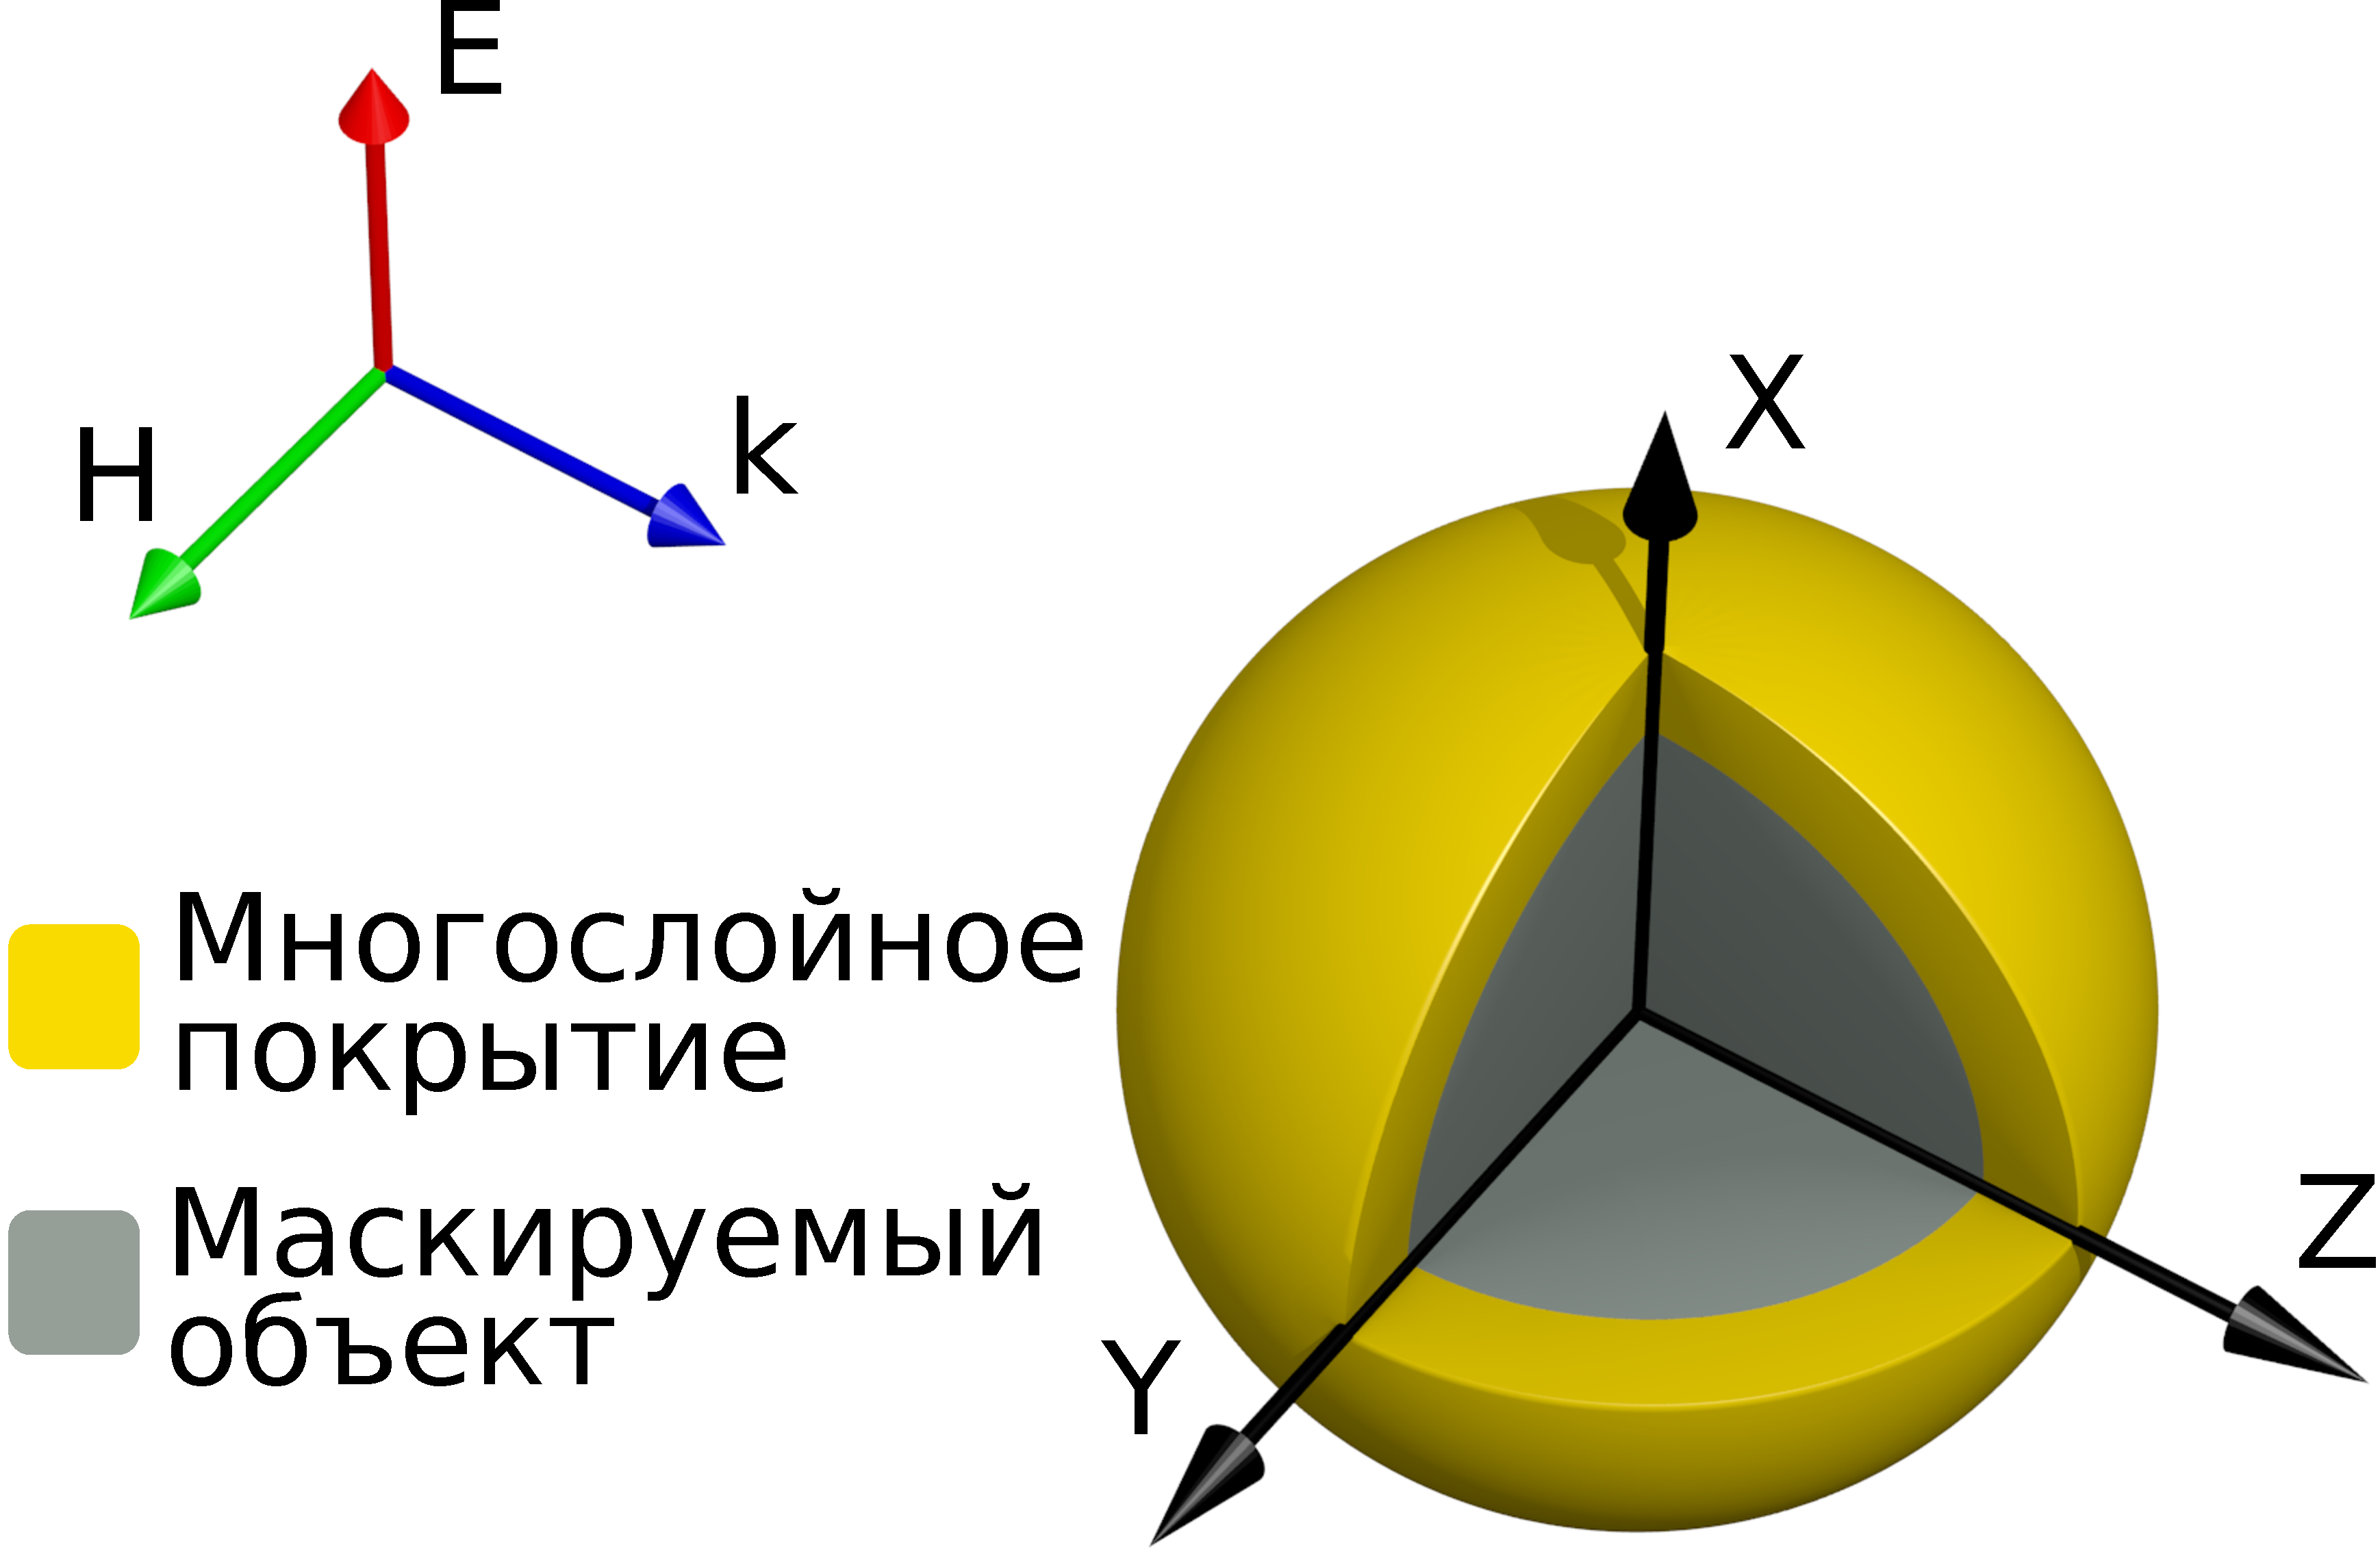
\includegraphics[width=0.47\textwidth]{model-view}%
    \caption{Схематическое изображение моделируемой системы: PEC сфера,
      окружённая многослойным диэлектрическим покрытием, и падающая
      плоская волна.\label{fig:model-view}}%
  }
\end{figure}
Малые потери были заданы в диэлектрических слоях (${k = 10 \time
  10^{-11}}$) для увеличения численной устойчивости моделирования Ми.


Мы исследовали возможное снижение RCS для диапазона толщины покрытия
от ${W = 0.02}$~см до ${W = 0.88}$~см с шагом 0.02~см с помощью серии
проходов оптимизации~(Рис.~\ref{fig:rcs-overview},%
 ~\ref{fig:rcs-overview-r14},~\ref{fig:rcs-overview-r42}).
\begin{figure}
  \center{
    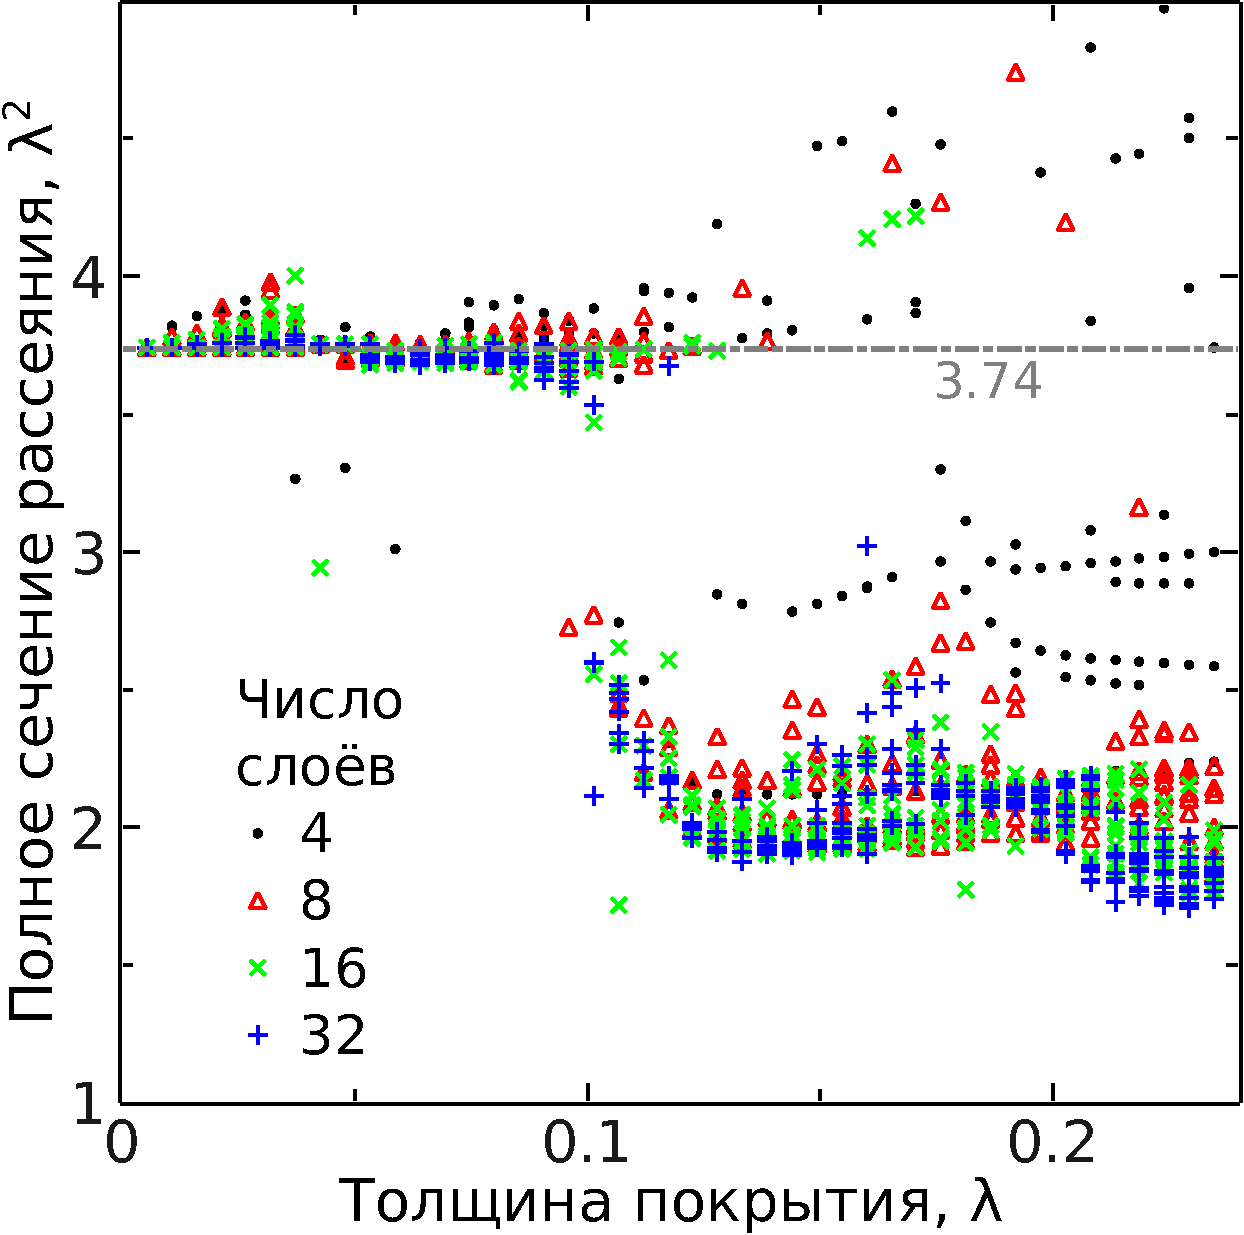
\includegraphics[width=0.47\textwidth]{rcs-overview}%
      \caption{Значение RCS после $\sim$2~000 проходов оптимизации в
        зависимости от толщины покрытия и числа слоёв в нём.  Мишень
        ${R = 2.81}$~см.  Каждая отметка на графике обозначает
        конечный результат одного прохода оптимизации. Типичное
        значение уменьшения RCS составило приблизительно
        -50\% относительно уровня непокрытой мишени, обозначенного
        пунктирной линией.
        \label{fig:rcs-overview}}%
    }
\end{figure}
\begin{figure}
    \center{
      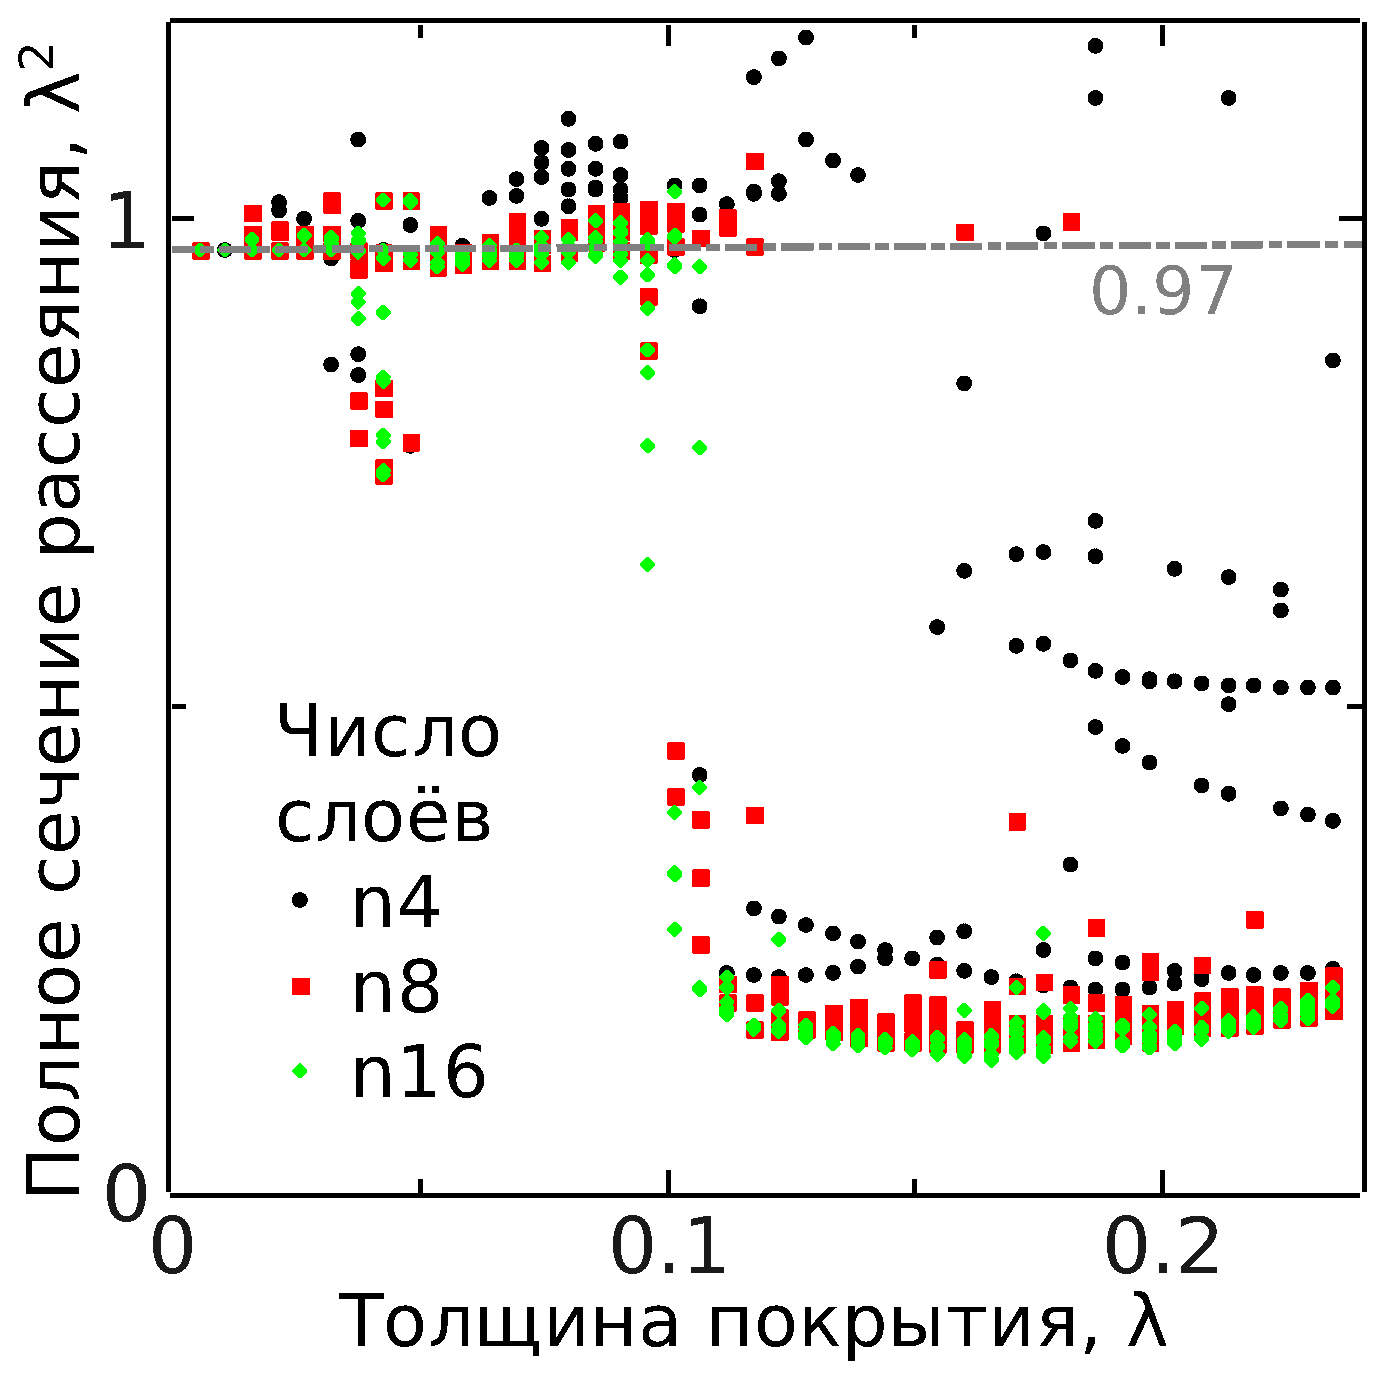
\includegraphics[width=0.47\textwidth]{rcs-overview-r14}%
      \caption{Аналогично Рис.~\ref{fig:rcs-overview} для мишени ${R =
          1.41}$~см.  Типичное значение уменьшения RCS составило
        приблизительно -85\%.  \label{fig:rcs-overview-r14}}%
    }
\end{figure}
\begin{figure}
    \center{
      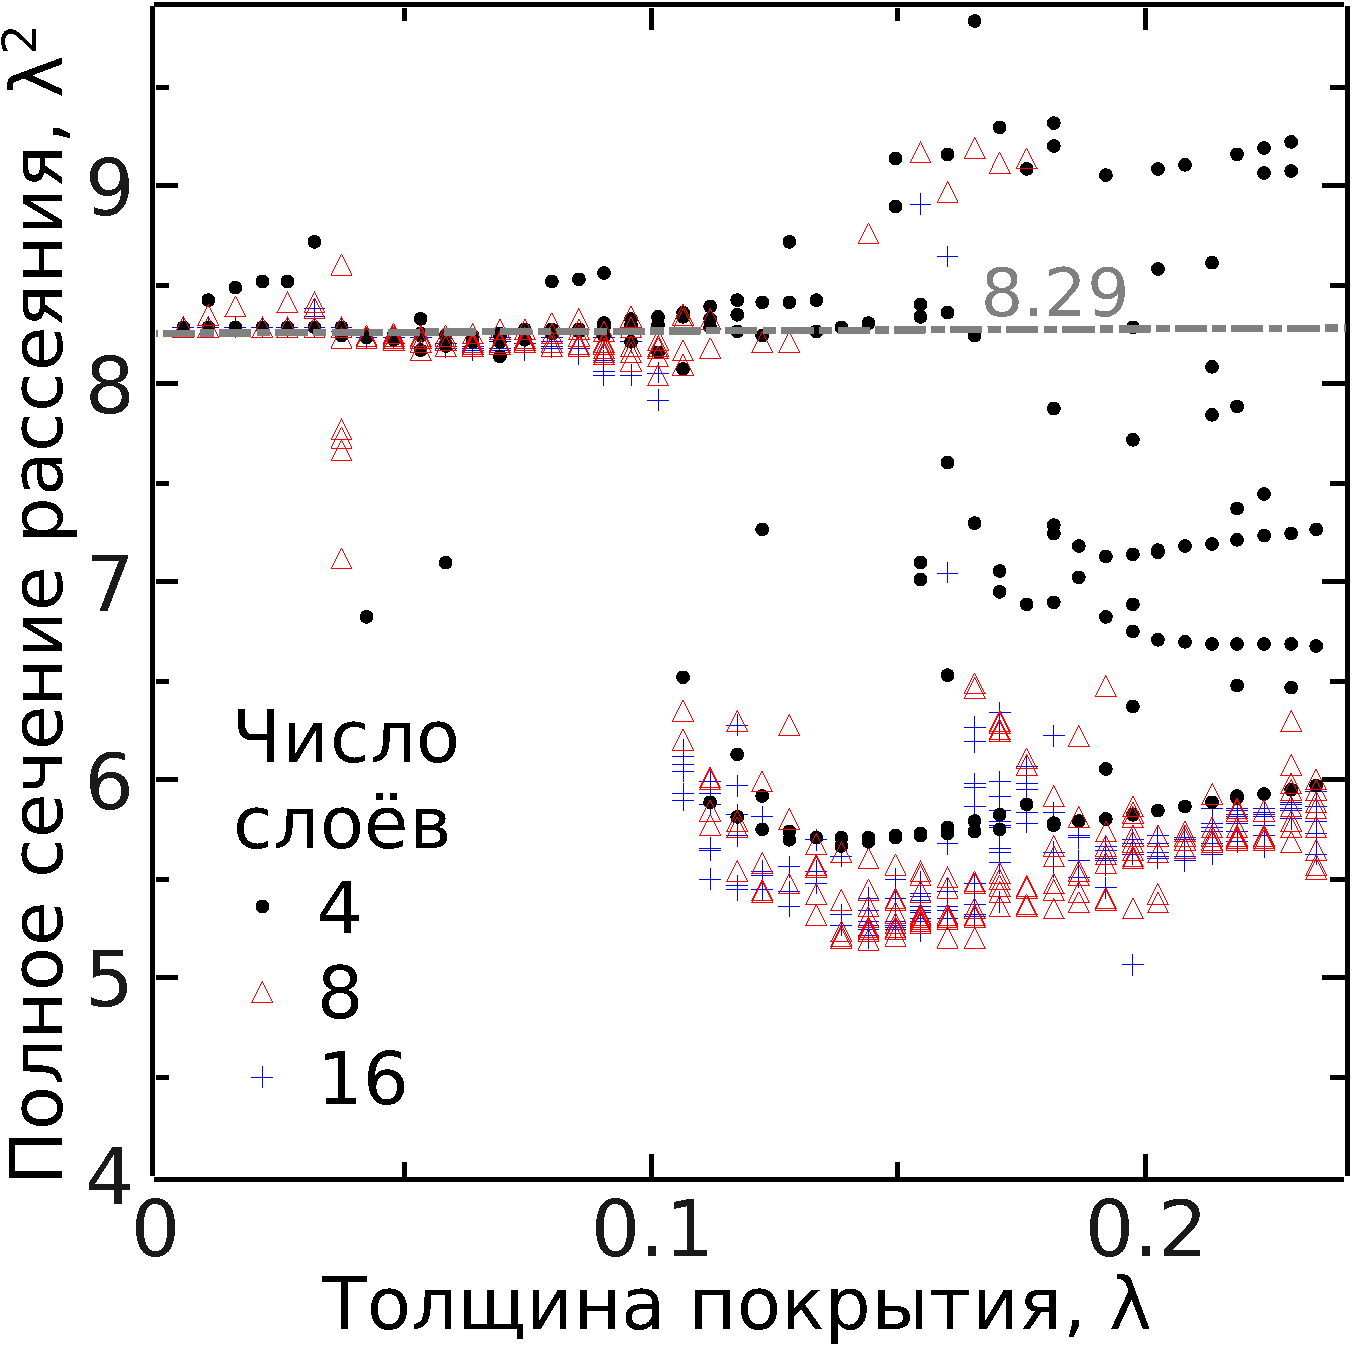
\includegraphics[width=0.47\textwidth]{rcs-overview-r42}%
      \caption{Аналогично Рис.~\ref{fig:rcs-overview} для мишени ${R =
          4.22}$~см.  Типичное значение уменьшения RCS составило
        приблизительно -35\%.  \label{fig:rcs-overview-r42}}%
    }
\end{figure}
Мы протестировали разбиение покрытия на 4, 8, 16 (для всех радиусов) и
32 слоя (для радиуса среднего размера). Существует некоторая
критическая величина общей толщины покрытия (${{\rmfamily W}\approx
  0.4}$~см), ниже которой оптимизатор был в состоянии найти только
несколько дизайнов с пониженной RCS относительно непокрытой мишени. Большинство
дизайнов с пониженной RCS имеют толщину покрытия выше критической.


Рассмотрим более подробно случай радиуса мишени ${R =
  2.81}$~см. Типичное снижение RCS относительно непокрытой мишени для
толщины выше критической составляет ${\approx -50\%}$ (в два
раза ниже). Непосредственно после превышения критической толщины
превалируют однодолинные
дизайны~(Рис.~\ref{fig:single-valley-index-design}, на всех графиках
дизайнов в настоящей статье мишень, представленная PEC сферой,
расположена слева, а открытое пространство справа).
\begin{figure}
  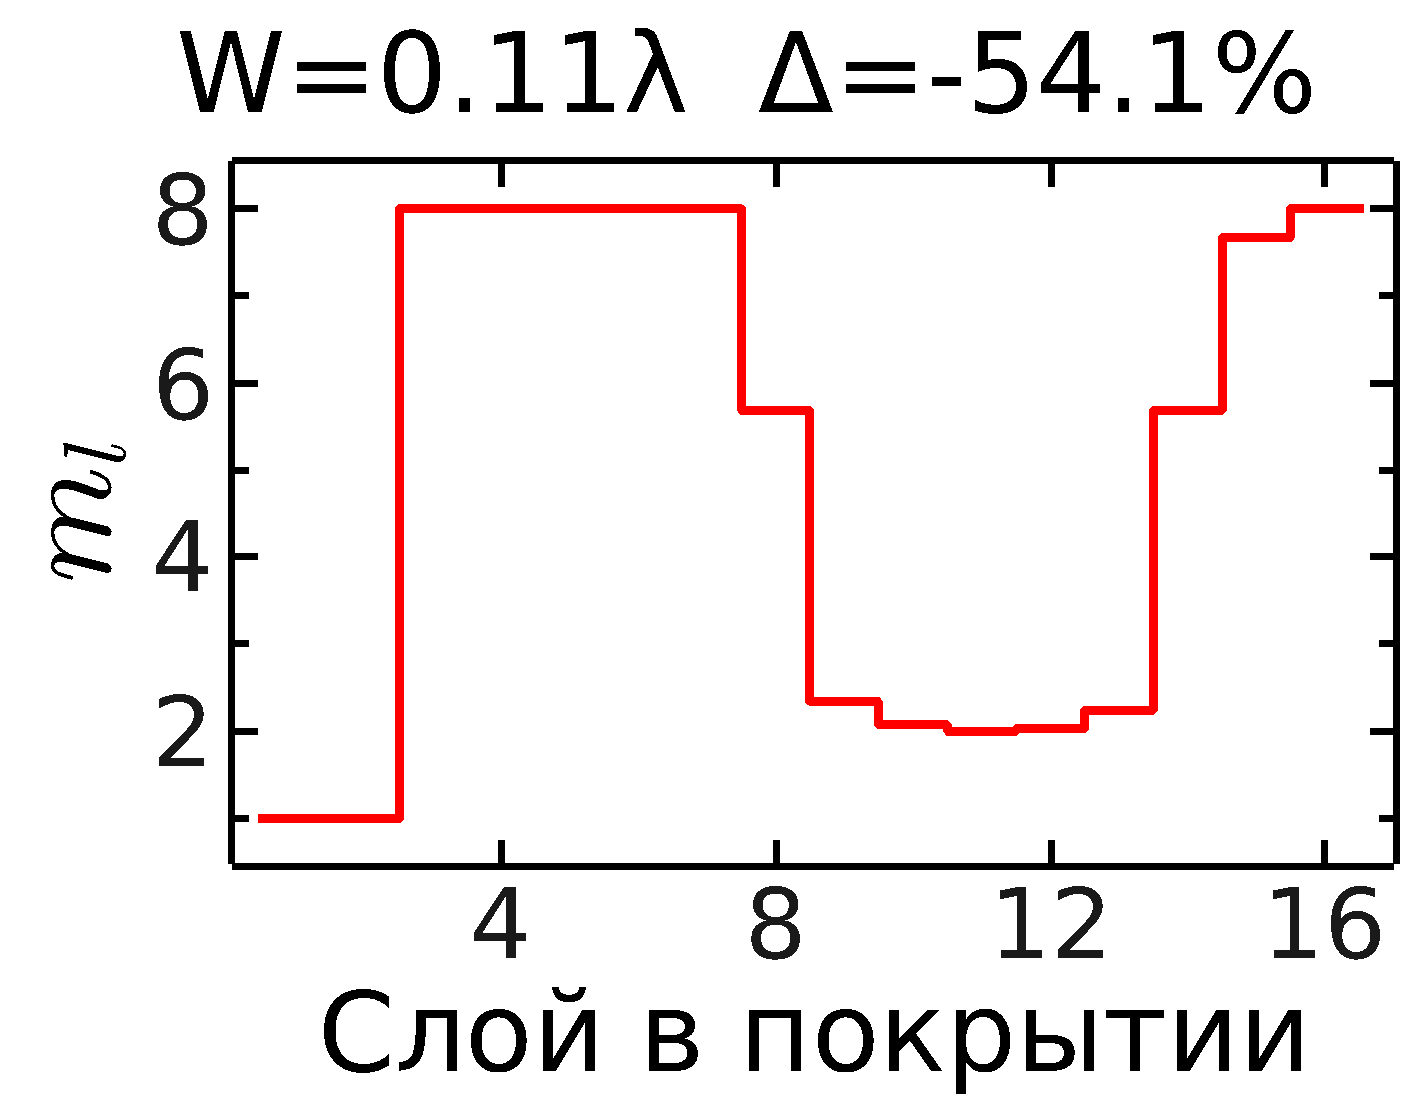
\includegraphics[width=0.47\textwidth]{w04-single-valley-index}%
  \caption{Профиль показателя преломления внутри покрытия:
    однодолинный дизайн.  ${W=0.4}$~cm
    $\Delta {\textrm RCS}=-54.1\%$.
    \label{fig:single-valley-index-design}}%
\end{figure}
Такие дизайны, как правило, начинаются с воздушного промежутка между
покрытием и мишенью из PEC, затем следует быстрое увеличение
показателя преломления до максимально допустимого. После нескольких
слоёв с высоким значением величина показателя преломления постепенно
идёт вниз и снова вверх, образуя долину с низким значением внутри двух
стенок с высоким значением. Минимальное значение показателя
преломления в долине обычно оказывается около двух. За второй стенкой
долины величина показателя преломления резко падает с высокого значения до
уровня воздуха.

Наряду с ростом толщины от ${\approx 0.62}$~см до ${\approx 0.78}$~см
происходит переход ~(Рис.~\ref{fig:transition}) от
однодолинного~(Рис.~\ref{fig:single-valley-index-design}) к
двухдолинному~(Рис.~\ref{fig:CST-index-design}) дизайну, где оба
дизайна сосуществуют при одной и той же толщине.

\begin{figure}
  \begin{minipage}[h]{0.235\textwidth}
    % W=0.62~cm $\Delta$RCS=-47.9\% \\
    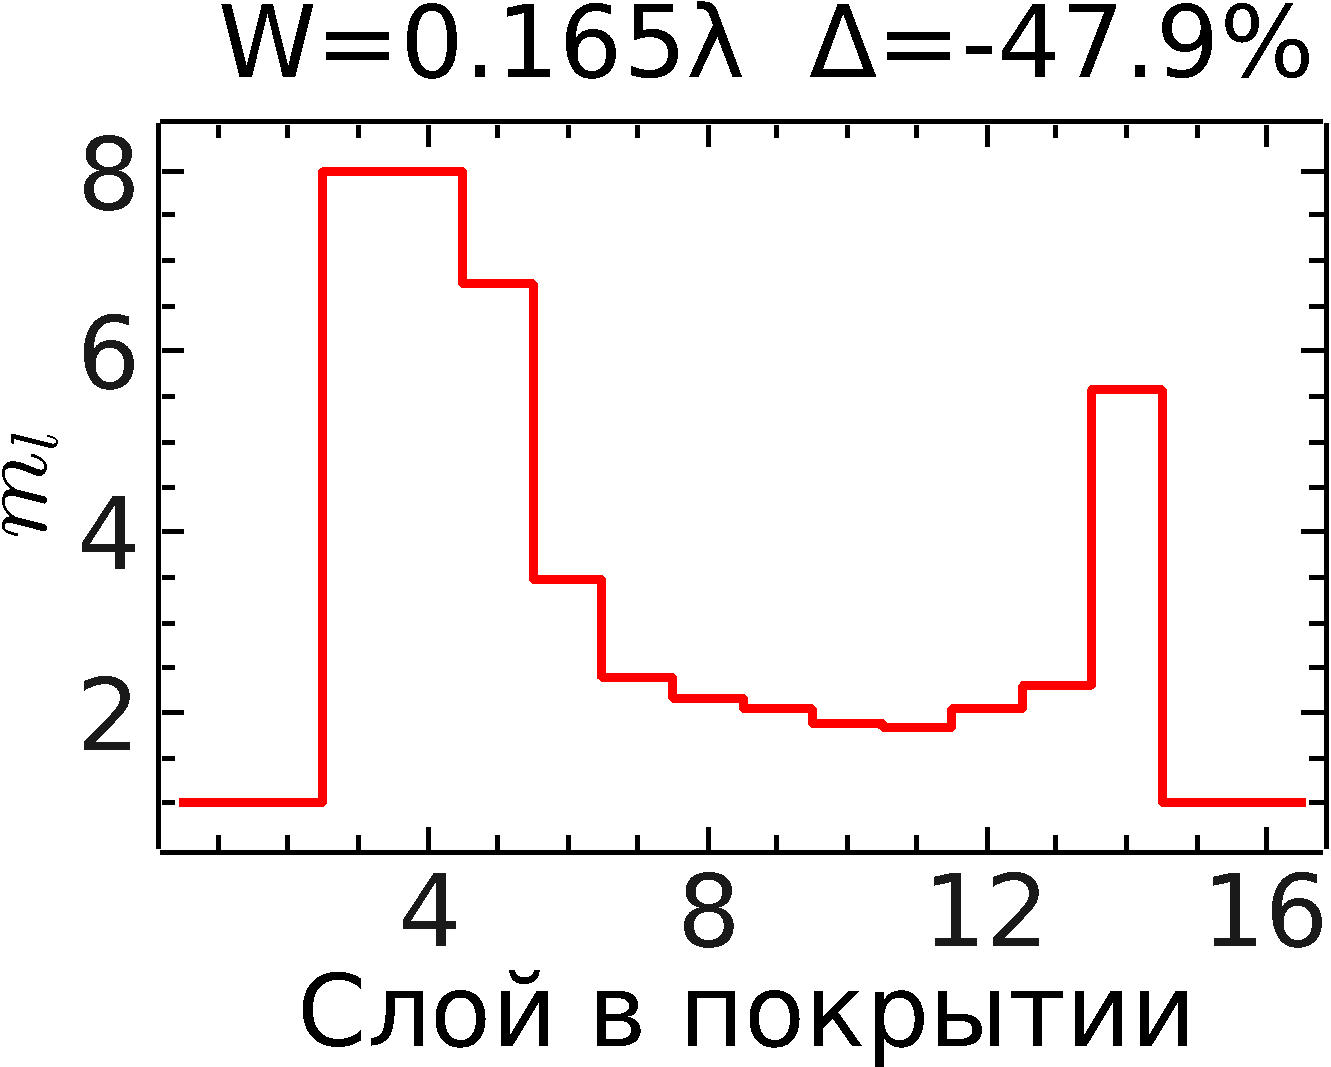
\includegraphics[width=0.99\textwidth]{w062-s-diff-479}
  \end{minipage}
  \hfill
  \begin{minipage}[h]{0.235\textwidth}
    % W=0.62~cm $\Delta$RCS=-32.3\%\\
    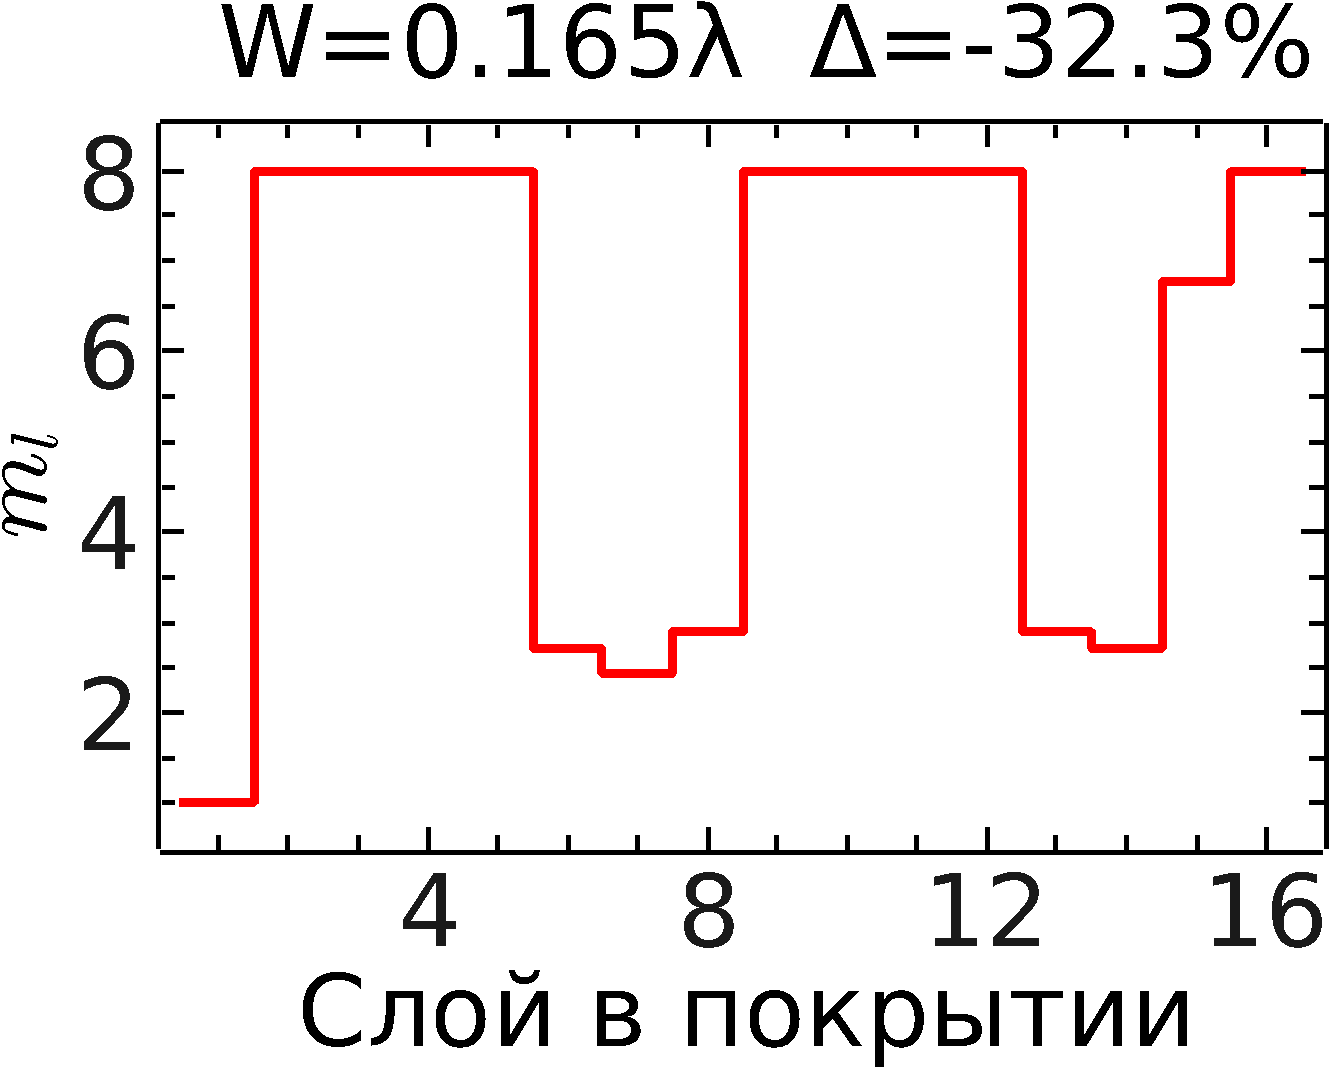
\includegraphics[width=0.99\textwidth]{w062-t-diff-323}
  \end{minipage}\\
  \vspace{7pt}
  % \vfill
  \begin{minipage}[h]{0.235\textwidth}
    % W=0.76~cm $\Delta$RCS=-46.9\%\\
    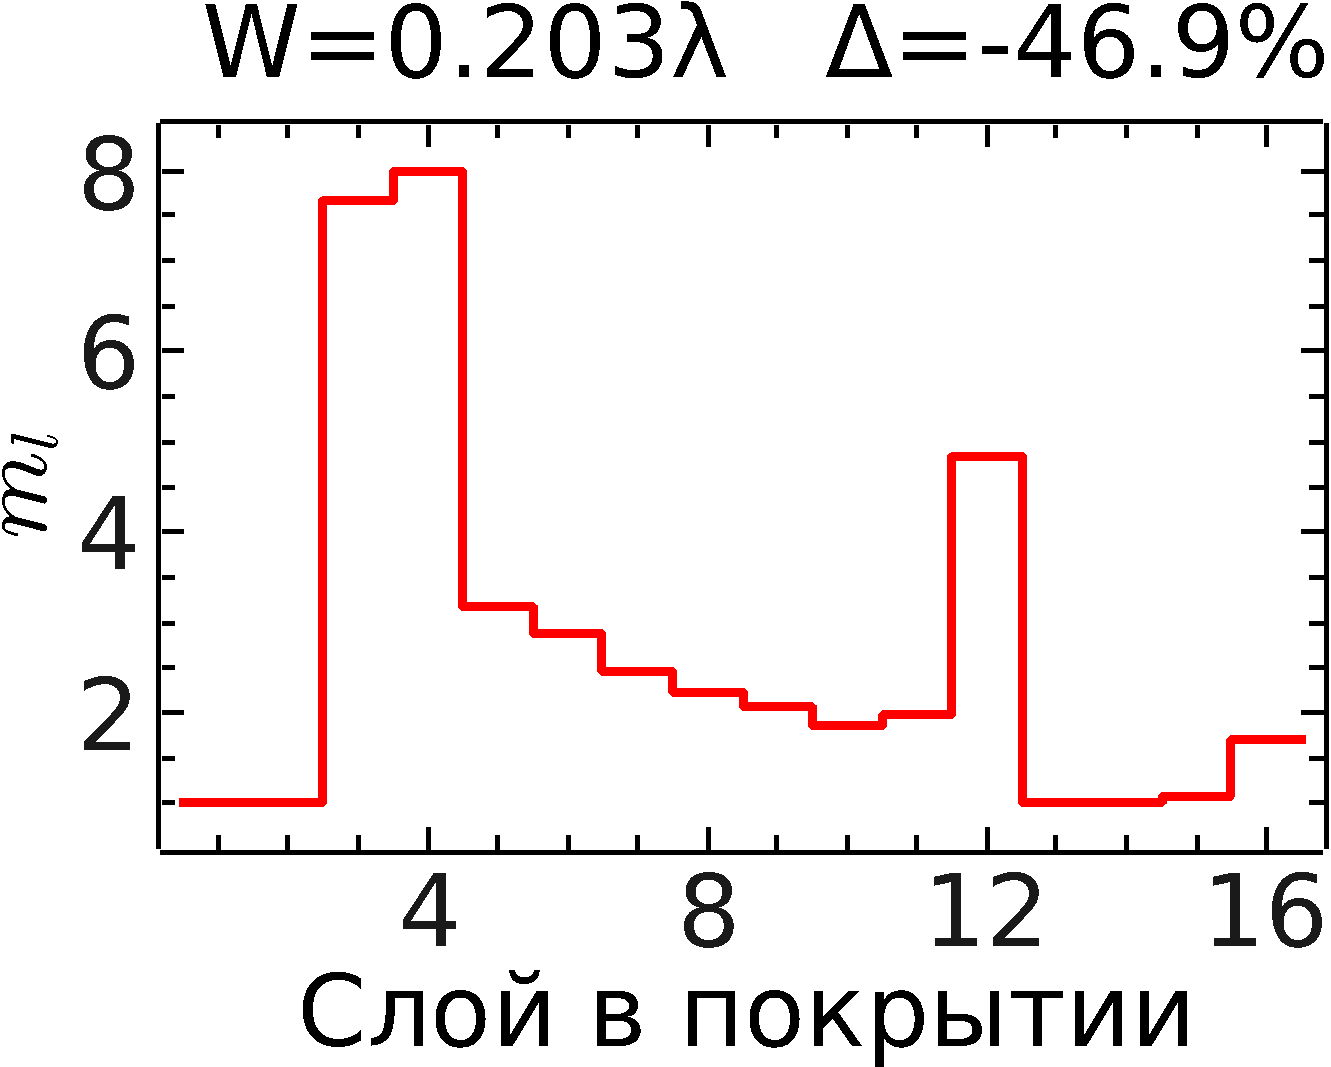
\includegraphics[width=0.99\textwidth]{w076-s-diff-469}
  \end{minipage}
  \hfill
  \begin{minipage}[h]{0.235\textwidth}
    % W=0.76~cm $\Delta$RCS=-41.9\%\\
    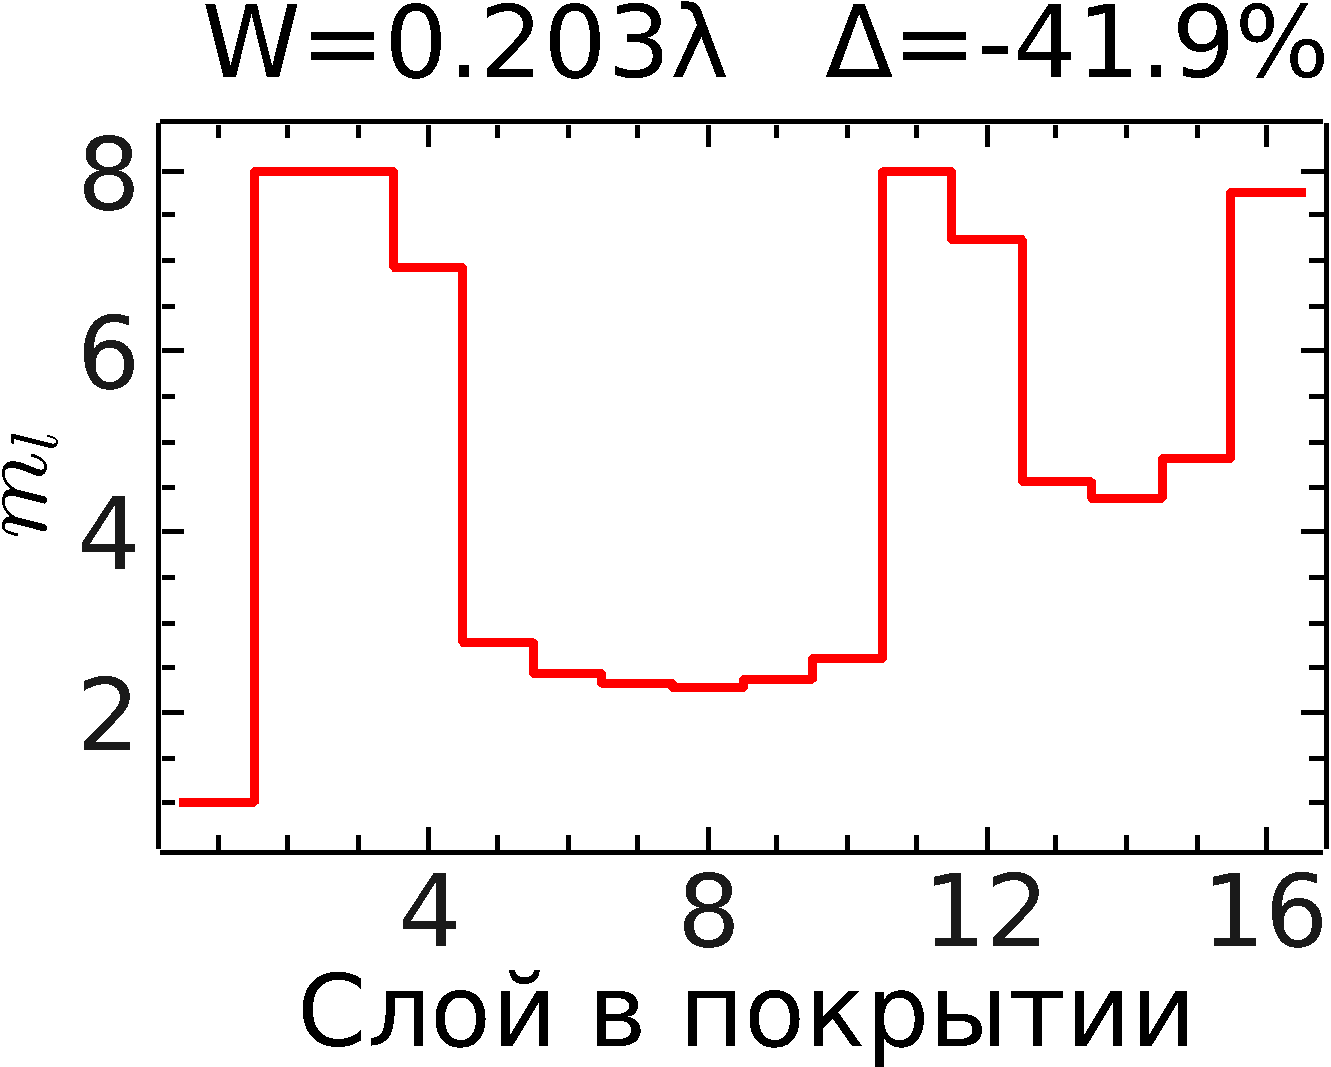
\includegraphics[width=0.99\textwidth]{w076-t-diff-419}
  \end{minipage}%
  \caption{Переход от однодолинного к двухдолинному дизайну. Каждый
    профиль показателя преломления был получен в отдельном проходе оптимизации.
    \label{fig:transition}}%
\end{figure}
\begin{figure}
  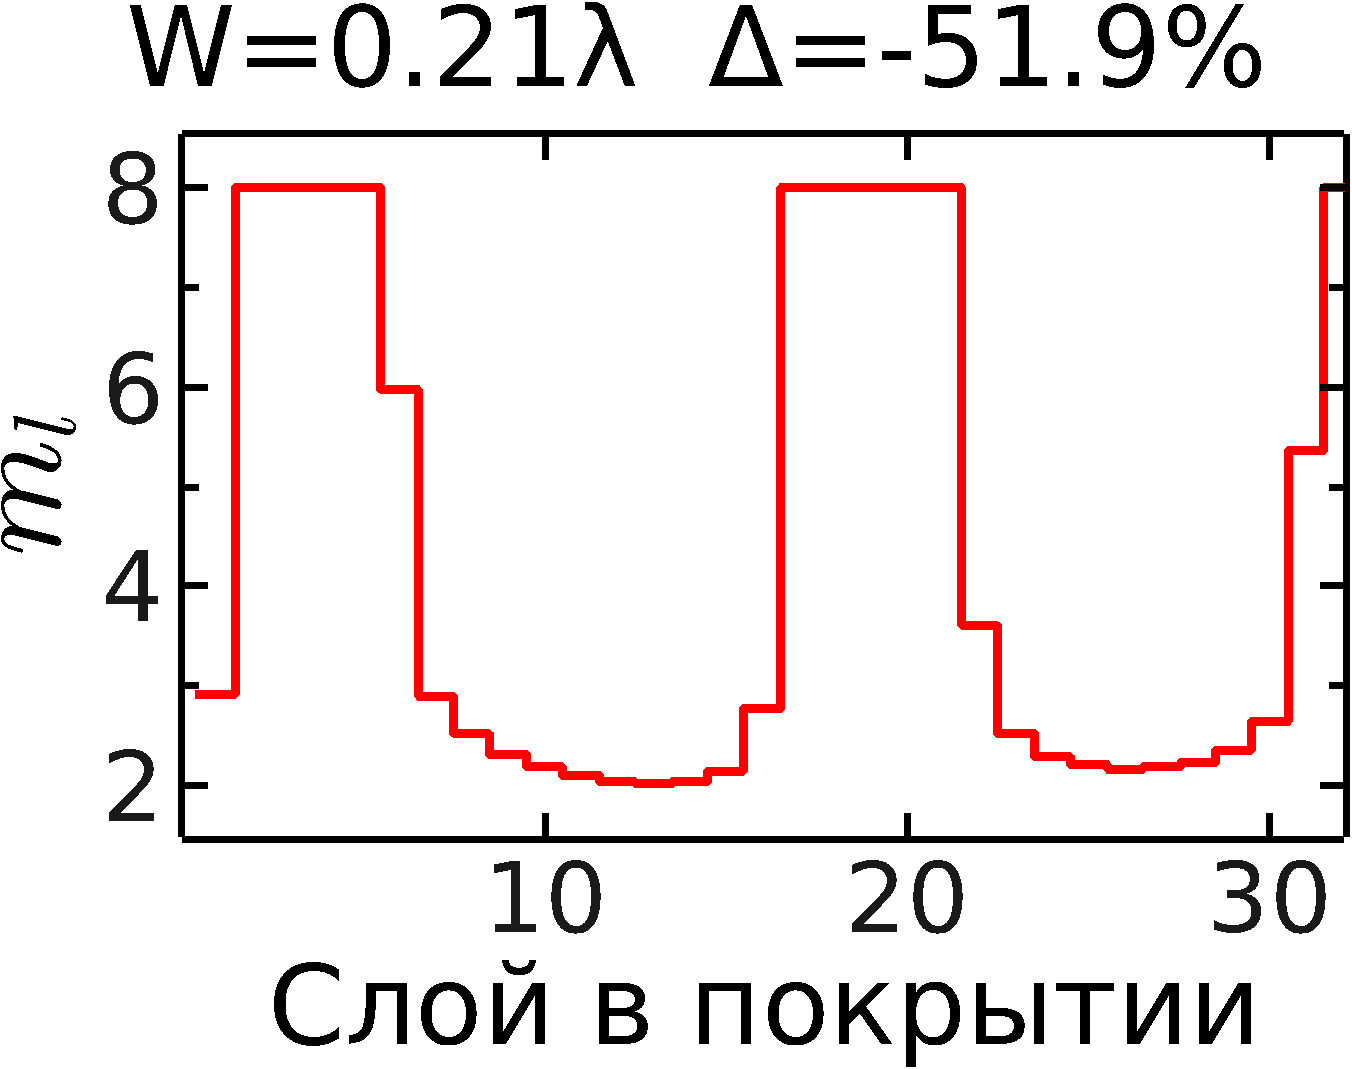
\includegraphics[width=0.47\textwidth]{w08-double-valley-index}%
  \caption{Двухдолинный дизайн показателя преломления, который был
    использован при моделировании в CST.  ${W=0.8}$~cm $\Delta {\textrm RCS}=-51.9\%$. 
    \label{fig:CST-index-design}}%
\end{figure}
Для толщины покрытия более ${\approx 0.68}$~см большинство дизайнов
имеет двухдолинную конфигурацию, немногие остальные не в полной мере
соответствуют однодолинной модели из-за наличия в покрытии внутреннего или
внешнего слоя с относительно высоким значением показателя
преломления. Для толщины выше ${\approx 0.78}$~м однодолинных дизайнов
обнаружено не было.

Во время перехода однодолинный дизайн представляется довольно
стабильным, поскольку он достиг наилучшего состояния. Двухдолинный
дизайн, видимо, ограничен допустимой толщиной покрытия. С увеличением
толщины покрытия ширина долин также увеличивается. Ширина внутренней
долины (которая ближе к PEC мишени) растёт быстрее. Это может быть
связано со следующим фактом: электромагнитное поле в покрытии в
основном сосредоточено во внутренних слоях
(Рис.~\ref{fig:CST-Ex}). Таким образом, дизайн внутренних слоёв
оказывает более сильное воздействие на итоговую RCS по сравнению с
наружными слоями; следовательно, внутренние слои имеют приоритет при
оптимизации.

Существенного дополнительного снижения RCS после перехода
не наблюдается. Мы полагаем, что также возможны многодолинные дизайны;
однако мы не смогли получить их из-за ограничений по времени и по
вычислительным мощностям. Была проведена быстрая попытка оптимизации
для толщины покрытия 2.4~см, для которой оптимизатор смог найти некий
дизайн~(Рис.~\ref{fig:thick}) с 54.3\% падением RCS.
\begin{figure}
  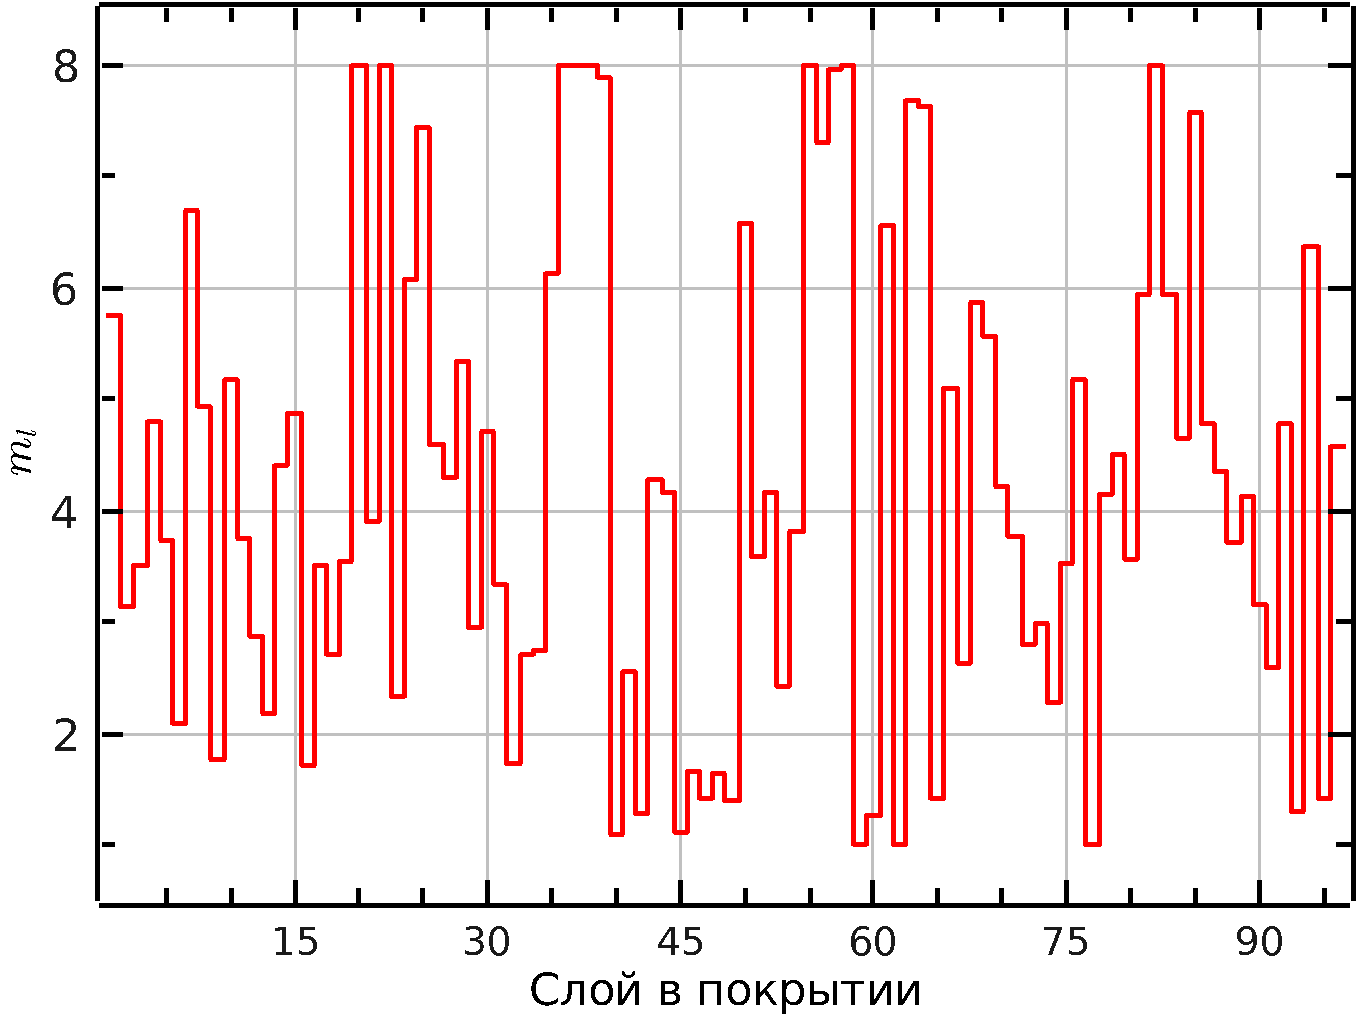
\includegraphics[width=0.47\textwidth]{w24-chaotic-index}%
  \caption{Хаотический дизайн для толщины покрытия $W=2.4$~cm
    $\Delta {\textrm RCS}=-54.3$\% после 10~000 поколений.
    \label{fig:thick}}%
\end{figure}
К сожалению, он выглядит довольно хаотично и не поддаётся простой
классификации.

%БЛОК 2

Необходимо отметить, что <<дёрганое>> поведение профиля показателя
преломления, хорошо видное в случае хаотического дизайна, может быть
частично обнаружено в случаях однодолинного и двухдолинных дизайнов,
описанных выше.  Это можно объяснить следующим образом: толщина
отдельного слоя внутри покрытий в десятки раз меньше длины волны (слои
являются субволновыми).  Таким образом, если поменять местами два
соседних слоя, то эффективное значение показателя преломления
поменяется слабо, и будет наблюдаться сопоставимая величина падения
RCS.  В случае, если разница в величине показателя преломления между
этими слоями оказывается достаточно большой, то будет наблюдаться
<<дёрганое>> поведения профиля показателя преломления.  Подобное
поведение тонких многослойных покрытий представляет
существенную сложность для любого алгоритма оптимизации, так как очень
похожие друг на друга с физической точки зрения системы оказываются
сильно удалены друг от друга в многомерном пространстве входных
параметров.  Иначе говоря, у весовой функции, используемой в качестве
критерия оптимизации, наблюдаются многочисленные локальные
минимумы.  Этот факт при использовании стохастического оптимизатора
приводит к тому, что конечный результат каждого прохода может
оказаться немного другим.  По этой причине для каждого набора входных
параметров выполнялась серия проходов оптимизации, а это, в свою
очередь, обусловило наличие нескольких отметок одного типа
(одно и то же количество слоёв в покрытии) для каждой исследованной
толщины покрытия~(Рис.~\ref{fig:rcs-overview},%
~\ref{fig:rcs-overview-r14},~\ref{fig:rcs-overview-r42}), отметки с
большим значением величины RCS обычно обладают более <<дёрганым>>
профилем показателя преломления.  В целом, несмотря на указанные
сложности, адаптивный метод дифференциальной эволюции воспроизводимо
находит дизайны  с уменьшенным рассеянием в выбранном диапазоне толщин
и числа слоёв в разбиении.

Как следует из Рис.~\ref{fig:rcs-overview}, разбиения покрытия на
четыре слоя оказывается недостаточным для достижения оптимальных
значений RCS.  Большинство дизайнов, обладающих RCS более 35~см$^2$ и
толщиной покрытия, превышающей критическую, используют разбиение на 4
слоя.  При этом разбиения на 8 слоёв оказывается достаточным для того,
чтобы получить результаты, сравнимые со случаями 16 и 32 слоёв
(особенно для диапазона толщин покрытия, соответствующих однодолинному
дизайну).  Тем не менее, у разбиения на 32 слоя есть небольшое
преимущество в случае большой толщины покрытия (${> 0.8}$~см).

Как было указано ранее, обнаружено небольшое число дизайнов с
маскирующим эффектом в случае толщины покрытия значительно меньше
критической.  Чтобы изучить такие дизайны мы провели дополнительную серию
оптимизаций (треугольники без заполнения на Рис.~\ref{fig:rcs-overview-thin}).
\begin{figure}
  \center{
    % Use pdfcrop to remove white margins
    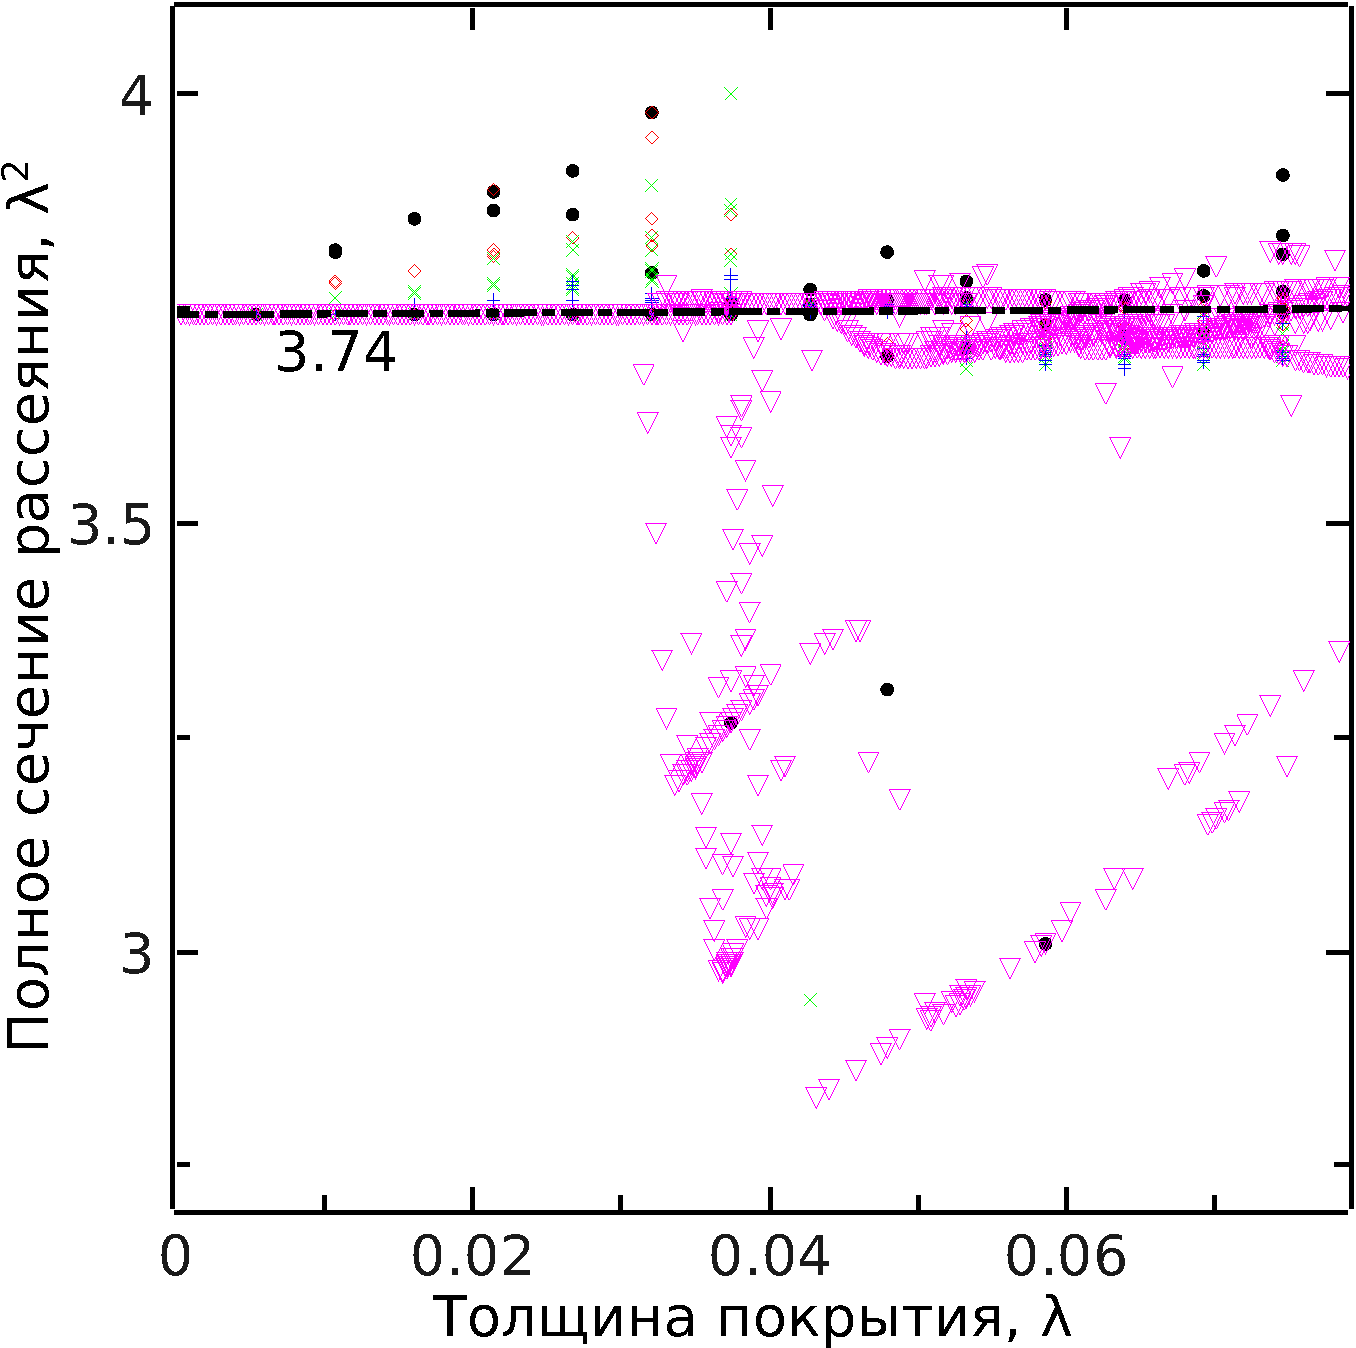
\includegraphics[width=0.47\textwidth]{rcs-overview-thin}%
      \caption{Увеличенная часть Рис.~\ref{fig:rcs-overview}) с
        дополнительными результатами оптимизации (треугольники без
        заполнения) для случая толщины покрытия меньше критической.
        Каждая отметка обозначает конечный результата одного прохода оптимизации.
        \label{fig:rcs-overview-thin}}%
  }
\end{figure}
Основываясь на ранее полученных результатах (а также по причине
ограниченных вычислительных ресурсов), мы использовали разбиение
только на 4 и 8 слоёв.  Для того чтобы добиться воспроизводимости
результатов, нам пришлось уменьшить шаг сканирования для толщины
покрытия и увеличить размер популяции в настройках оптимизатора.
Несмотря на это, всего лишь 218 проходов оптимизации из $\sim$4~000
смогли достичь значения RCS менее 50~см$^2$.  Лучший дизайн достиг
-24\% падения RCS для толщины покрытия 0.162~см.  Аналогичные дизайны
для сверхтонких покрытий, полученные в разных независимых прогонах
оптимизации, образуют хорошо различимые зависимости при изменении
толщины на Рис.~\ref{fig:rcs-overview-thin}.  Тем не менее, похоже, что
маскирующий эффект в таких покрытиях основан на несколько другом
физическом принципе, отличном от предлагаемого в настоящей работе, и
может быть дополнительно изучен впоследствии.

\section{Полноволновое моделирование}

Мы провели компьютерное моделирование различных дизайнов с помощью
пакета CST Microwave Studio 2013.  Полученные результаты обладают
набором общих особенностей, в иллюстративных целях мы выбрали
двухдолинный дизайн (Рис.~\ref{fig:CST-index-design}, а также его спектры Рис.~\ref{fig:CST-design-spectra}).
\begin{figure}
  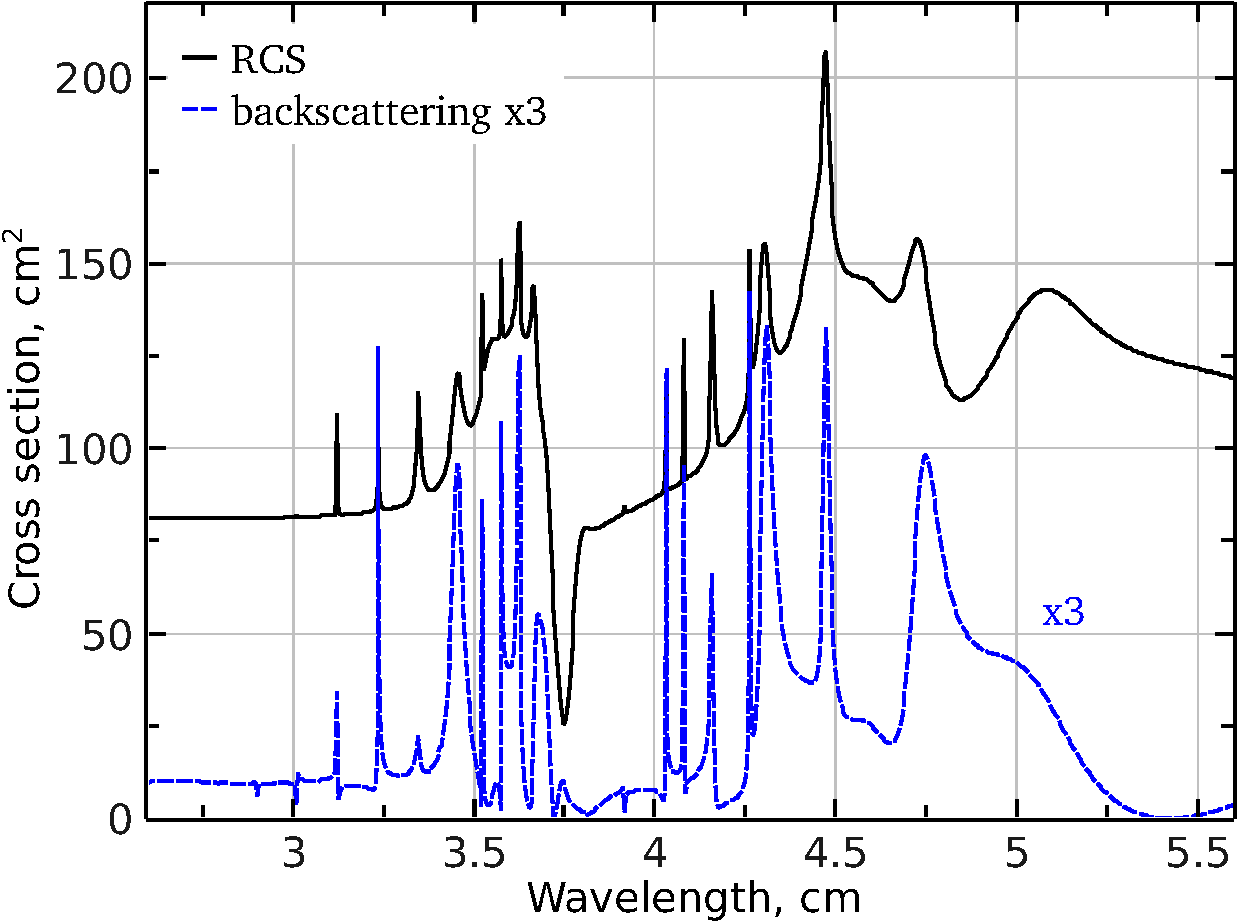
\includegraphics[width=0.47\textwidth]{w08-spectra}%
  \caption{Спектры RCS и сечения обратного рассеяния, полученные в
    Scattnlay~\cite{pena_scattering_2009} для двухдолинного дизайна,
    использованного при моделировании в пакете CST. Масштаб сечения
    для кривой обратного рассеяния увеличен в три раза.  Толщина
    покрытия $W=0.8$~см. Относительно непокрытой мишени $\Delta {\textrm
      RCS}=-51.9$\% при длине волны $\lambda=3.75$~cm.     %TODO add    bare target spectra
    \label{fig:CST-design-spectra}}%
  % TODO Zero-backscattering can be disscused with Limonov and
  % Rybin. They can do additional review of the paper.
\end{figure}
% CST rcs 25.4445 Mie 25.3412
Результаты компьютерного моделирования в пакете CST подтвердили
результаты расчётов с использованием теории Ми (25.44~см$^2$ и
25.34~см$^2$ соответственно).

Стационарное распределение поля (амплитуда  и фаза на
Рис.~\ref{fig:CST-Ex}) на частоте ${f = 8}$~ГГц были получены при
использовании алгоритмов CST в частотной области для разупорядоченной
тетрагональной сетки.
\begin{figure}
  \center{
    % Use pdfcrop to remove white margins
    \begin{minipage}[h]{0.47\textwidth}
      a)\hfill
      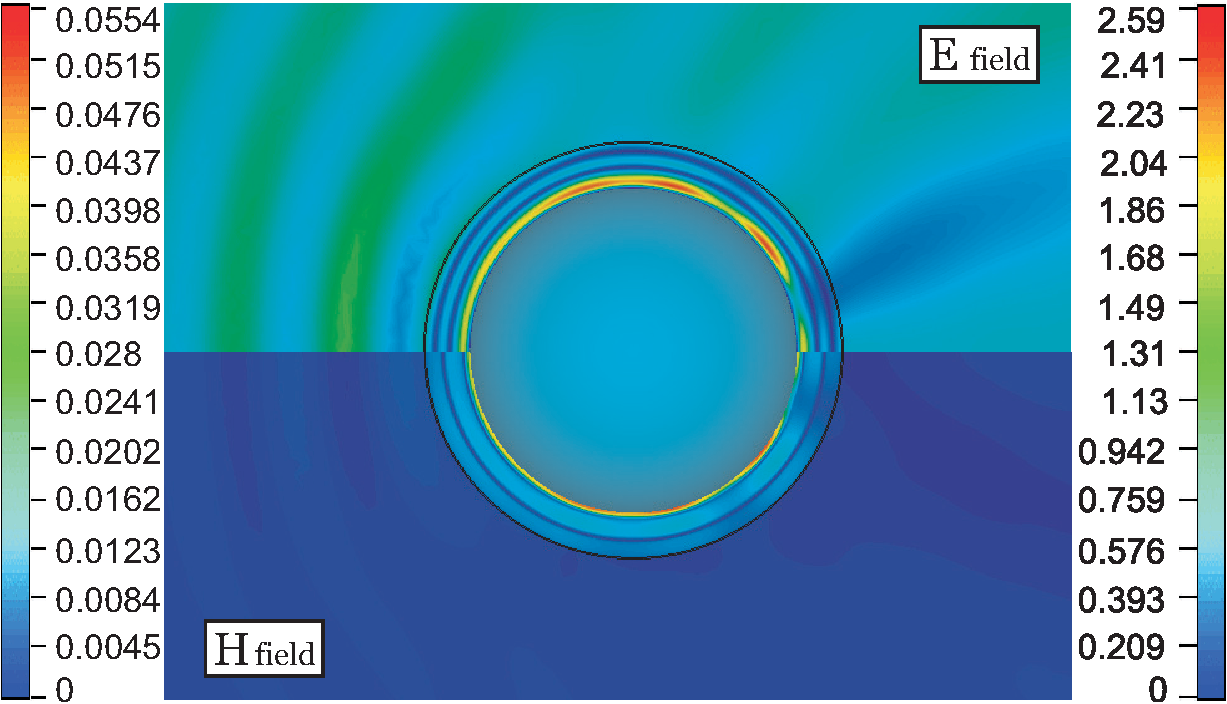
\includegraphics[width=0.95\textwidth]{W08-planeYZ-E-H-abs}%
    \end{minipage}\\%
    \begin{minipage}[h]{0.47\textwidth}
      b)\hfill
      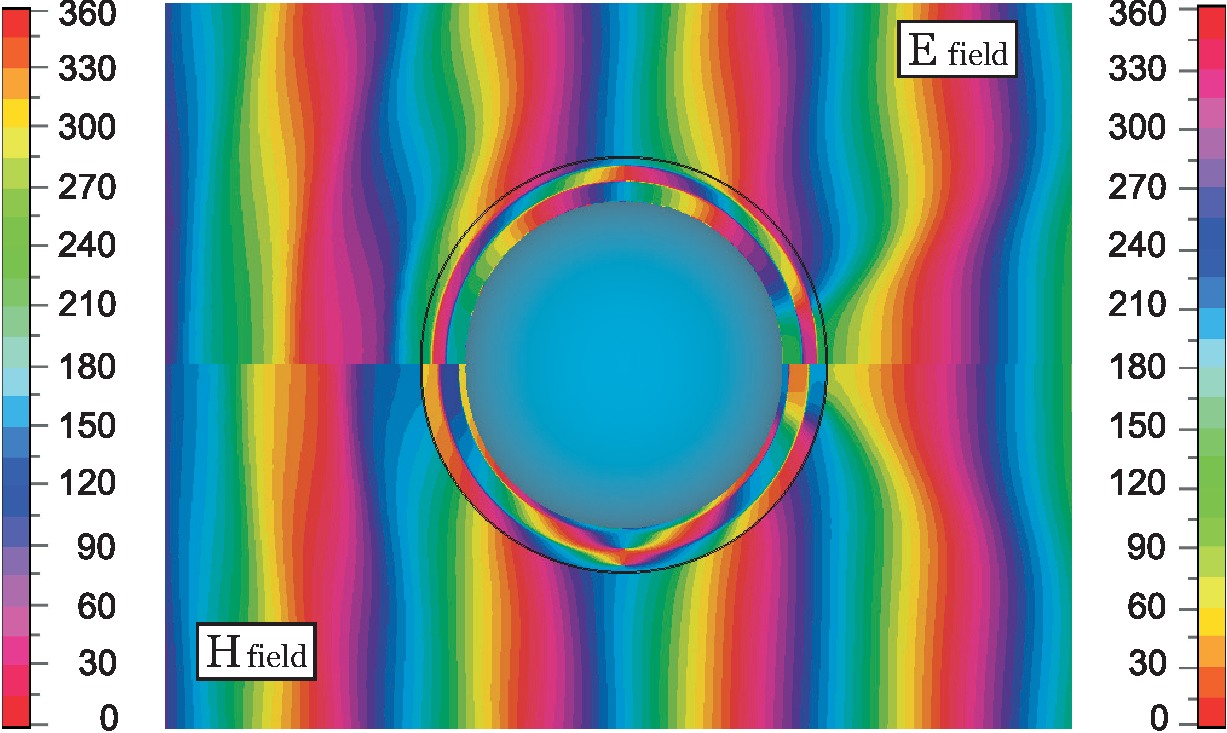
\includegraphics[width=0.95\textwidth]{W08-planeYZ-E-H-phase}%
    \end{minipage}%
      \caption{Амплитуда (a) и фаза (b) электрического (верхняя
        половина) и магнитного (нижняя половина) поля для
        двухдолинного дизайна. Окружности чёрного цвета обозначают
        границы внешнего слоя в покрытии.   Плоскость рисунка
        перпендикулярна плоскости поляризации электрического поля в
        падающей волне и проходит через центр мишени.  Амплитуда
        магнитного поля (левая шкала) измеряется в А/м, электрического
        поля (правая шкала) в В/м.  Фаза измеряется в градусах.
        \label{fig:CST-Ex}}%
  }
\end{figure}
Полное число ячеек в сетке составило около 4-х миллионов.  Для того
чтобы уменьшить моделируемый объём, мы использовали плоскости
симметрии.  Было выбрано открытое граничное условие с отражательной
способностью -40~dB.  Источник плоской волны расположен слева от
сферической мишени, плоскость поляризации электрического поля
перпендикулярна плоскости рисунка.

Необходимо отметить несколько особенностей распределения поля внутри
покрытия. 1) Электромагнитное поле в основном сконцентрировано во
внутренних слоях покрытия. 2) Присутствует нечто вроде антикорреляции
между минимумами и максимумами пространственного распределения
амплитуд электрического и магнитного полей: максимум электрического
поля соответствует минимуму магнитного и наоборот. 3) Существуют
тонкие <<переключающие>> слои с быстрым изменением фазы.  Прохождение
волны сквозь эти слои в радиальном направлении приводит к перевороту
её фазы на половину периода, далее идёт толстый слой перевёрнутой
фазы.  Положение <<переключающих>> слоёв совпадает с минимумами
амплитуды того поля, чья фаза переворачивается.

Давайте проследим за электрическим и магнитным полем, проходящим
через <<переключающие>> слои.  Такие слои можно эффективно
рассматривать как области резкого замедления распространения поля,
причиной которого является интерференция падающей и рассеянной волны.
Кроме того, плоскость постоянной фазы в области между
<<переключающими>> слоями имеет предпочтительное направление движения
в тангенциальном направлении.  Таким образом, один из возможных путей,
по которому может пойти падающая волна, выглядит следующим образом:
волна замедляется при прохождении сквозь <<переключающий>> слой, далее
она движется в радиальном направлении вдоль этого слоя,
замедляется ещё раз, проходя <<переключающий>> слой в обратном
направлении, и покидает покрытие.  Вследствие использованного дизайна
показателя преломления  набег фазы волны, проходящей внутри покрытия,
относительно волны, которая двигалась снаружи, оказывается в точности
равен полному периоду волны.  В результате поле, которое
распространялось подобным образом, не возмущает плоскость постоянной
фазы за мишенью.  Указанное поведение можно также трактовать с позиций
теории компенсации рассеяния~\cite{alu} со следующим дополнением.  В
нашем случае наличие антипараллельных векторов локальной
поляризуемости  вызвано наличием <<переключающих>> слоёв, приводящих к
изменению направления вектора электрического поля на противоположное.

В случае двухдолинного дизайна возникает два <<переключающих>> слоя.
Внешний слой работает указанным выше образом, внутренний слой работает
аналогично, но с небольшим отличием.  Набег фазы волны, проходящей
через внутренний слой, оказывается равен двум периодам.

Предложенное физическое описание механизма уменьшения полного сечения
рассеяния позволяет сделать простое предсказание.  При рассмотрении
указанных дизайнов во временной области установление стационарного
распределения амплитуды поля в области геометрической тени займёт
больше времени в случае двухдолинного дизайна по сравнению с
однодолинным.  

\section{Заключение}

Адаптивный метод дифференциальной эволюции может быть успешно
использован для оптимизации полностью диэлектрических многослойных
покрытий в целях снижения рассеяния от сферических мишеней.  Были
найдены профили с оптимальным показателем преломления для различных
размеров мишени и толщин покрытия.  Были обнаружены одно- и
двухдолинные дизайны, которые оказались оптимальными для различных
геометрических параметров покрытия.  Для заданной максимальной
величины показателя преломления существует некая критическая толщина
покрытия, до который крайне тяжело найти дизайны покрытия с
маскирующим эффектом.  Для толщины покрытия больше критической
возникает переход от однодолинного дизайна к двухдолинному.  После
перехода существенного уменьшения RCS не наблюдалось.  Мы
предполагаем, что также возможно существование многодолинных дизайнов,
однако мы не смогли их обнаружить по причине ограниченных
вычислительной мощности и времени.  Полученные дизайны дают
возможность для реализации маскировки без использования магнитных и
анизотропных метаматериалов.
   


TODO перестановки в пространстве для хаотического дизайна.

\underline{\textbf{Третья глава}} посвящена исследованию свойств
многослойных сферических маскирующих покрытий. Схематическое
изображение модели приводится на рисунке~\ref{img:scattering}а. Для
заданного соотношения длины волны и диаметра маскируемого объекта с
помощью оптимизатора подбирались параметры многослойного покрытия
таким образом, чтобы уменьшить полное сечение рассеяния.  Покрытие
разбивалось на фиксированное количество слоёв одинаковой толщины, а в
качестве параметров оптимизации использовались показатели преломления
каждого слоя.  Результат оптимизации в виде зависимости полного
сечения рассеяния от количества слоёв и общей толщины покрытия
приводится на рисунке~\ref{img:scattering}б.
\begin{figure}[t]
  \begin{minipage}[ht]{0.45\linewidth}        
    \center{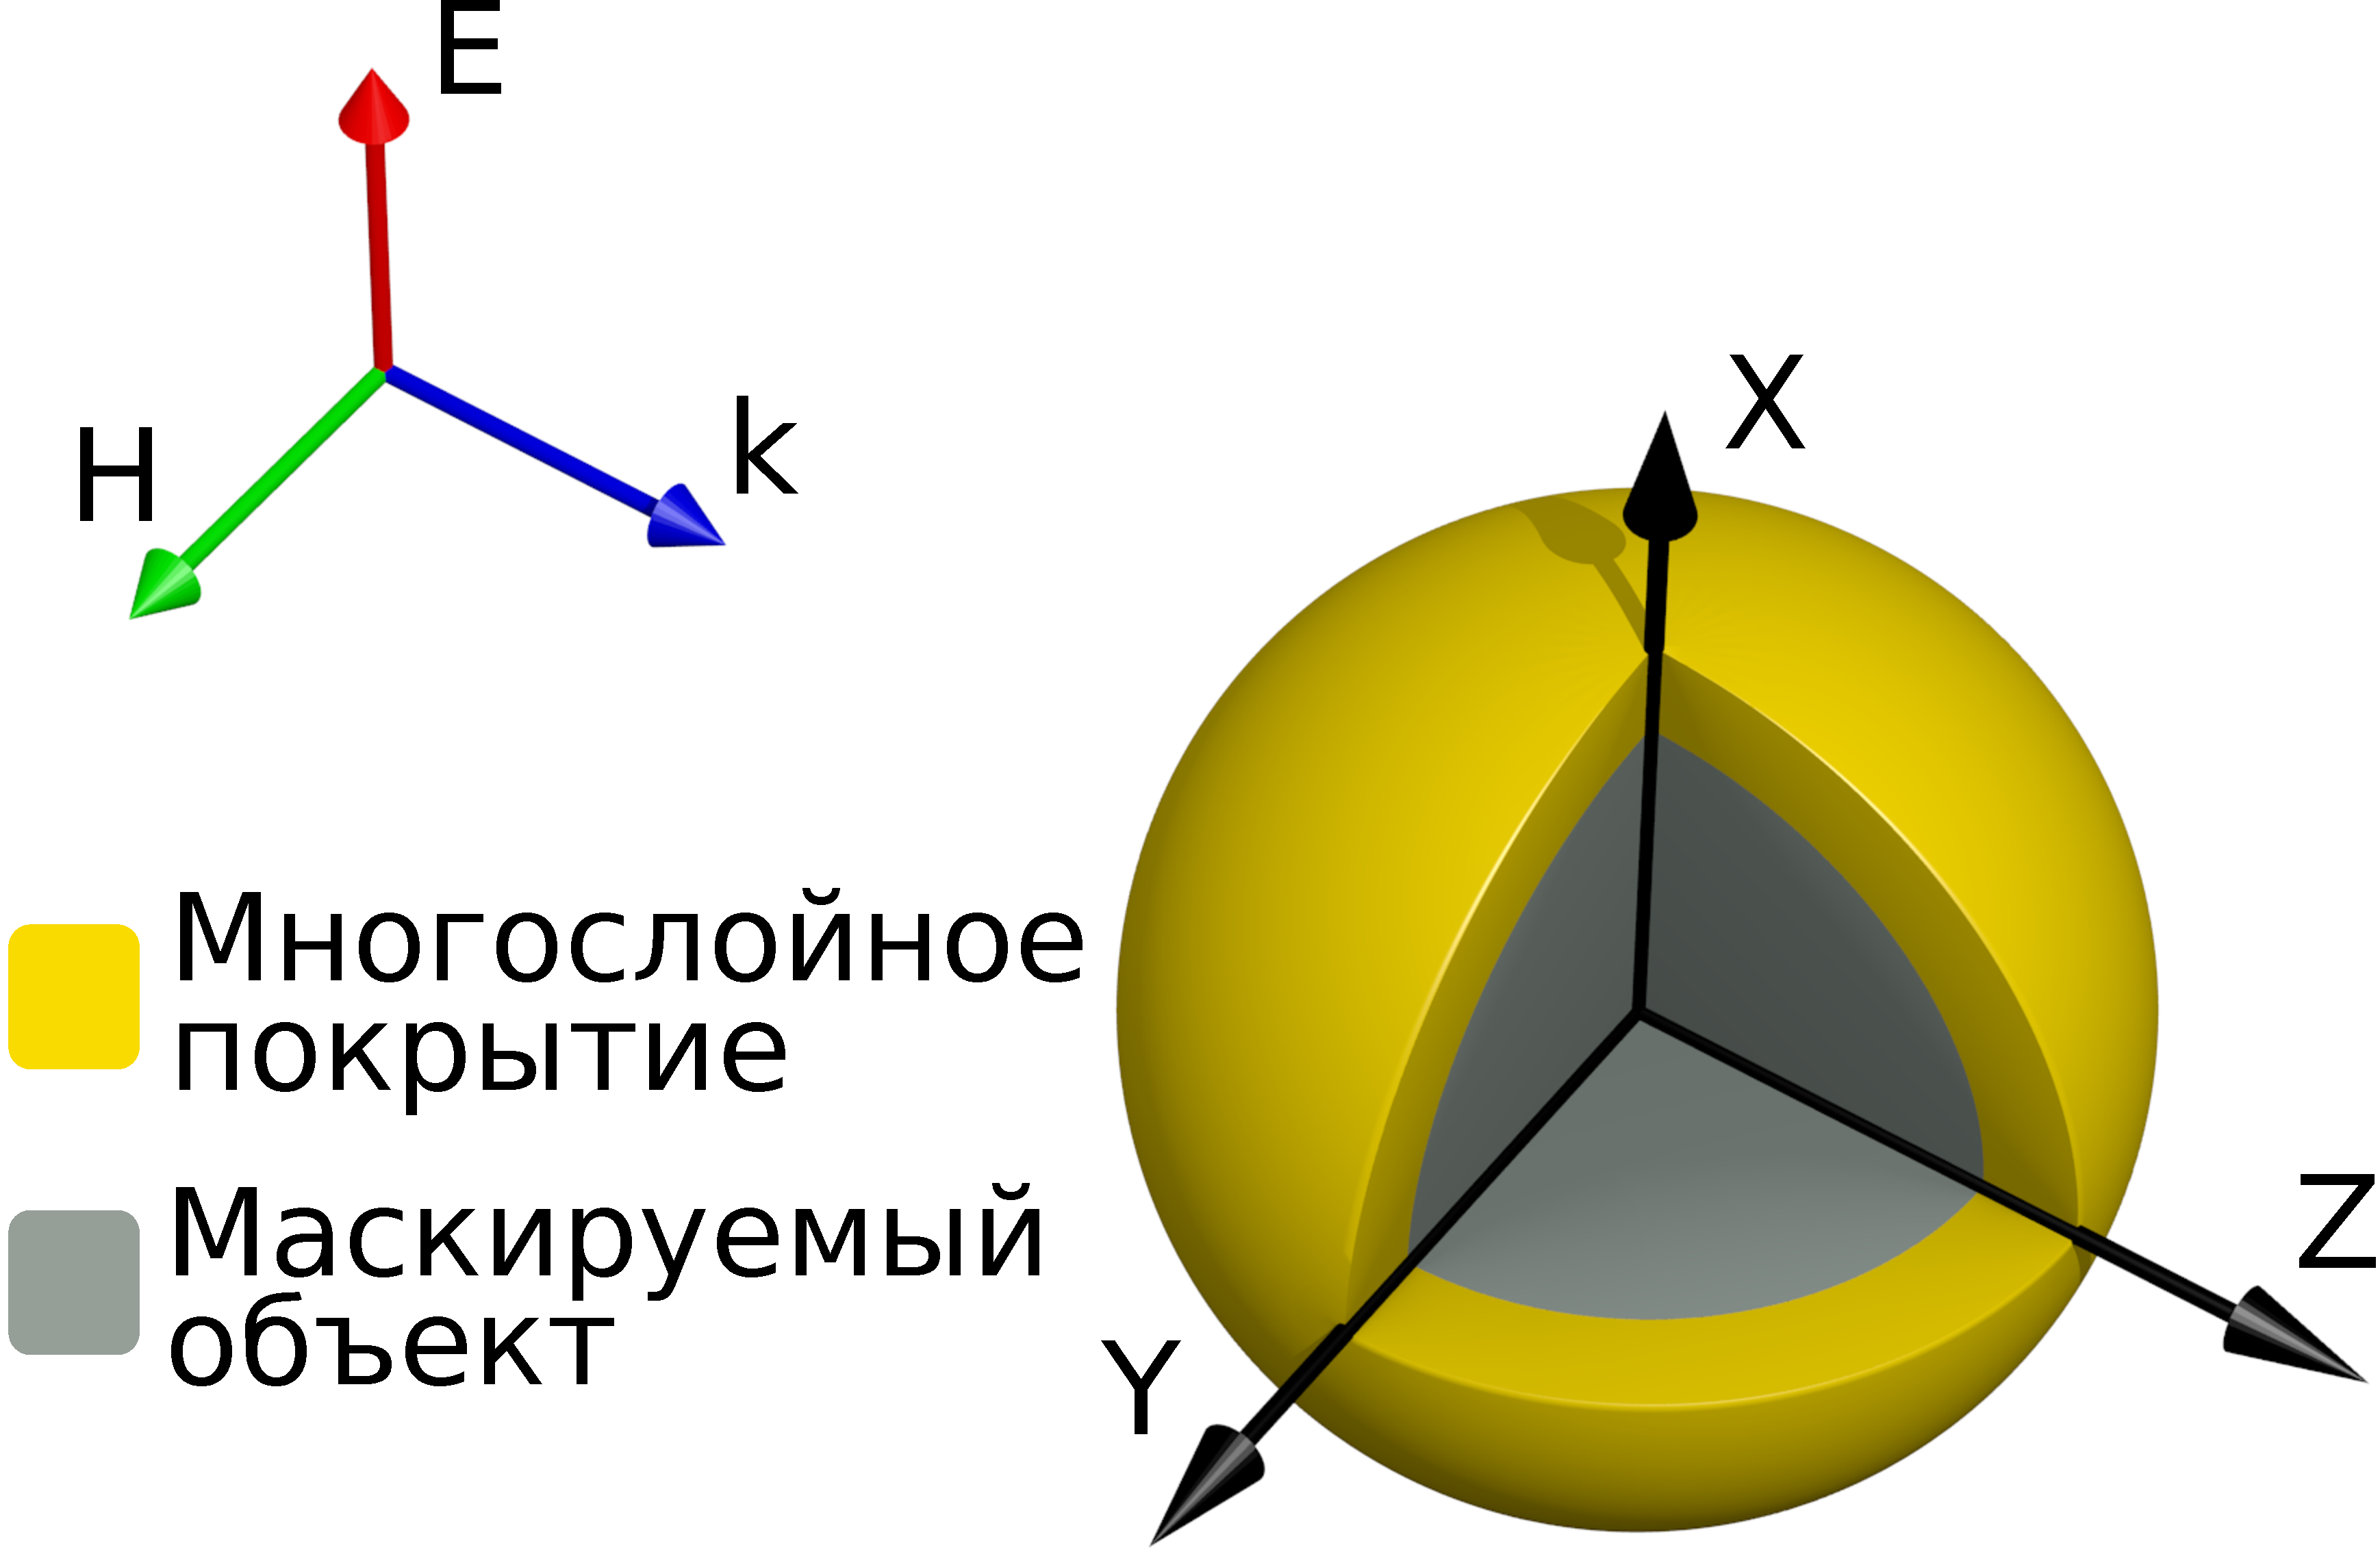
\includegraphics[width=0.95\linewidth]{model-view}}
  \end{minipage}
  \hfill
  \begin{minipage}[ht]{0.54\linewidth}
    \center{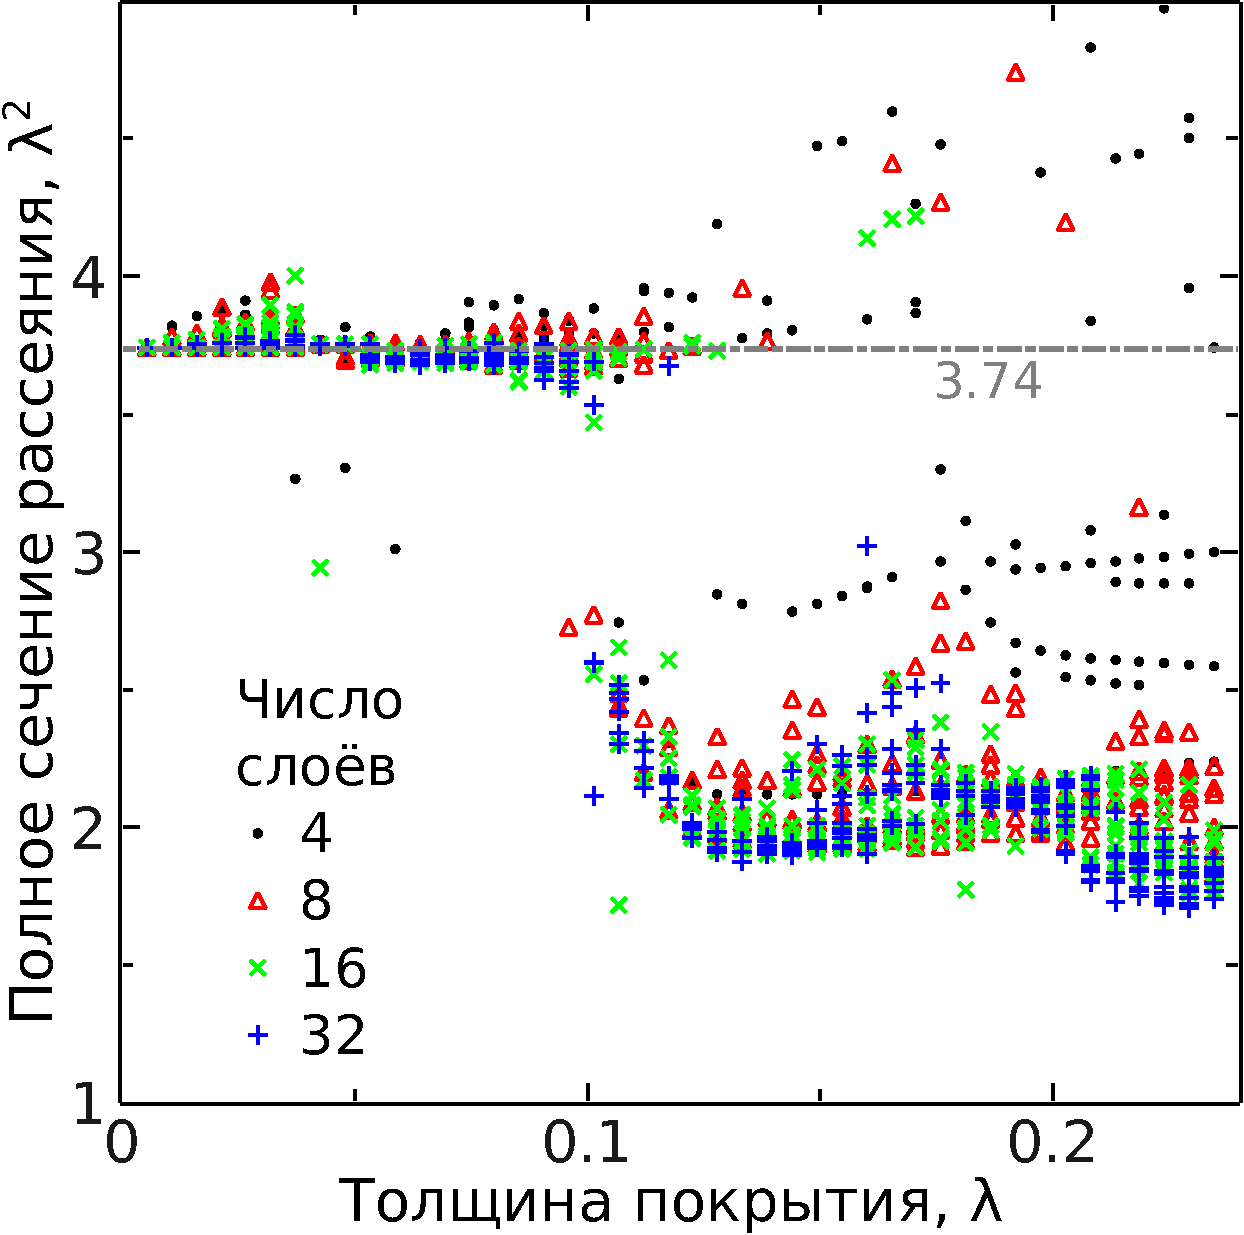
\includegraphics[width=0.95\linewidth]{rcs-overview} }
  \end{minipage}\\
  \vspace{0.3em}\\
  \begin{minipage}[ht]{0.45\linewidth}        
    \center{а)}
  \end{minipage}
  \hfill
  \begin{minipage}[ht]{0.54\linewidth}
    \center{б)}
  \end{minipage}

  \caption{(a) Схематическое изображение изучаемой системы: маскируемый
    объект -- сфера из идеального проводящего материала внутри
    многослойного диэлектрического покрытия и падающая
    электромагнитная волна. (б) 
    Результат работы оптимизатора для объекта диаметром $1.5\lambda$.
    % (TODO use plot for $\lambda/1.5$?)
    Каждая отметка на графике соответствует одному дизайну покрытия,
    полученному в результате минимизации рассеяния. При толщине
    покрытия $>0.15\lambda$ рассеяние можно уменьшить в $\sim 2$
    раза.}
  \label{img:scattering}  
\end{figure}
\begin{figure}[p]
  \begin{minipage}[ht]{0.32\linewidth}
    \center{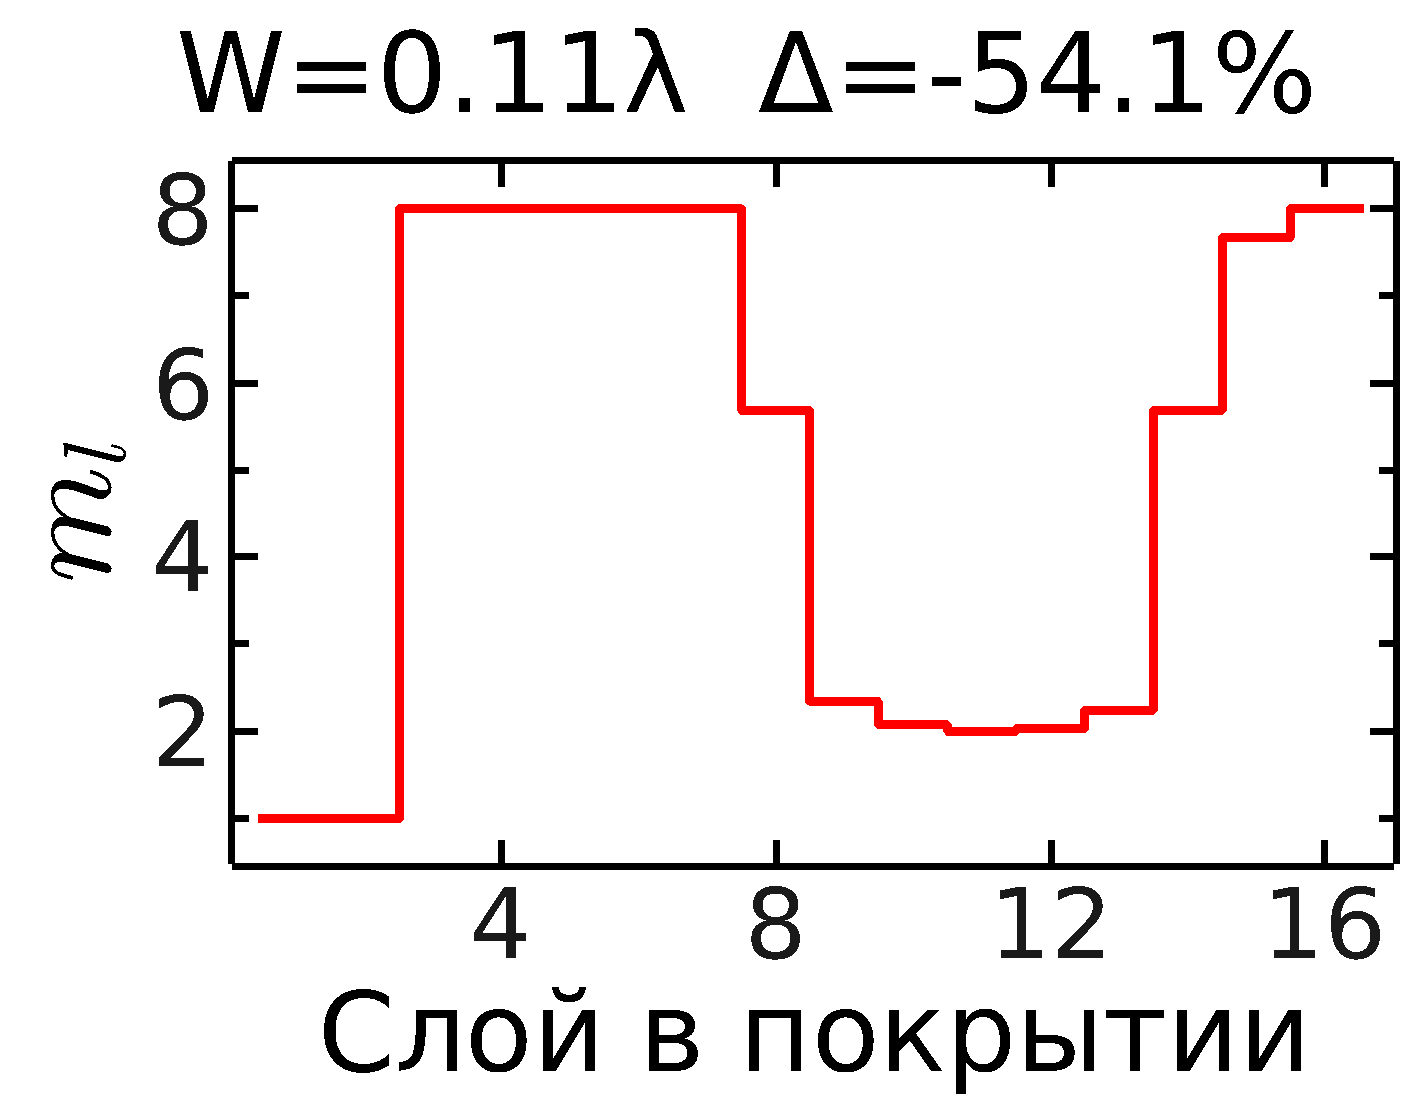
\includegraphics[width=0.95\linewidth]{w04-single-valley-index} \\ а)}
  \end{minipage}
  \hfill
  \begin{minipage}[ht]{0.32\linewidth}
    \center{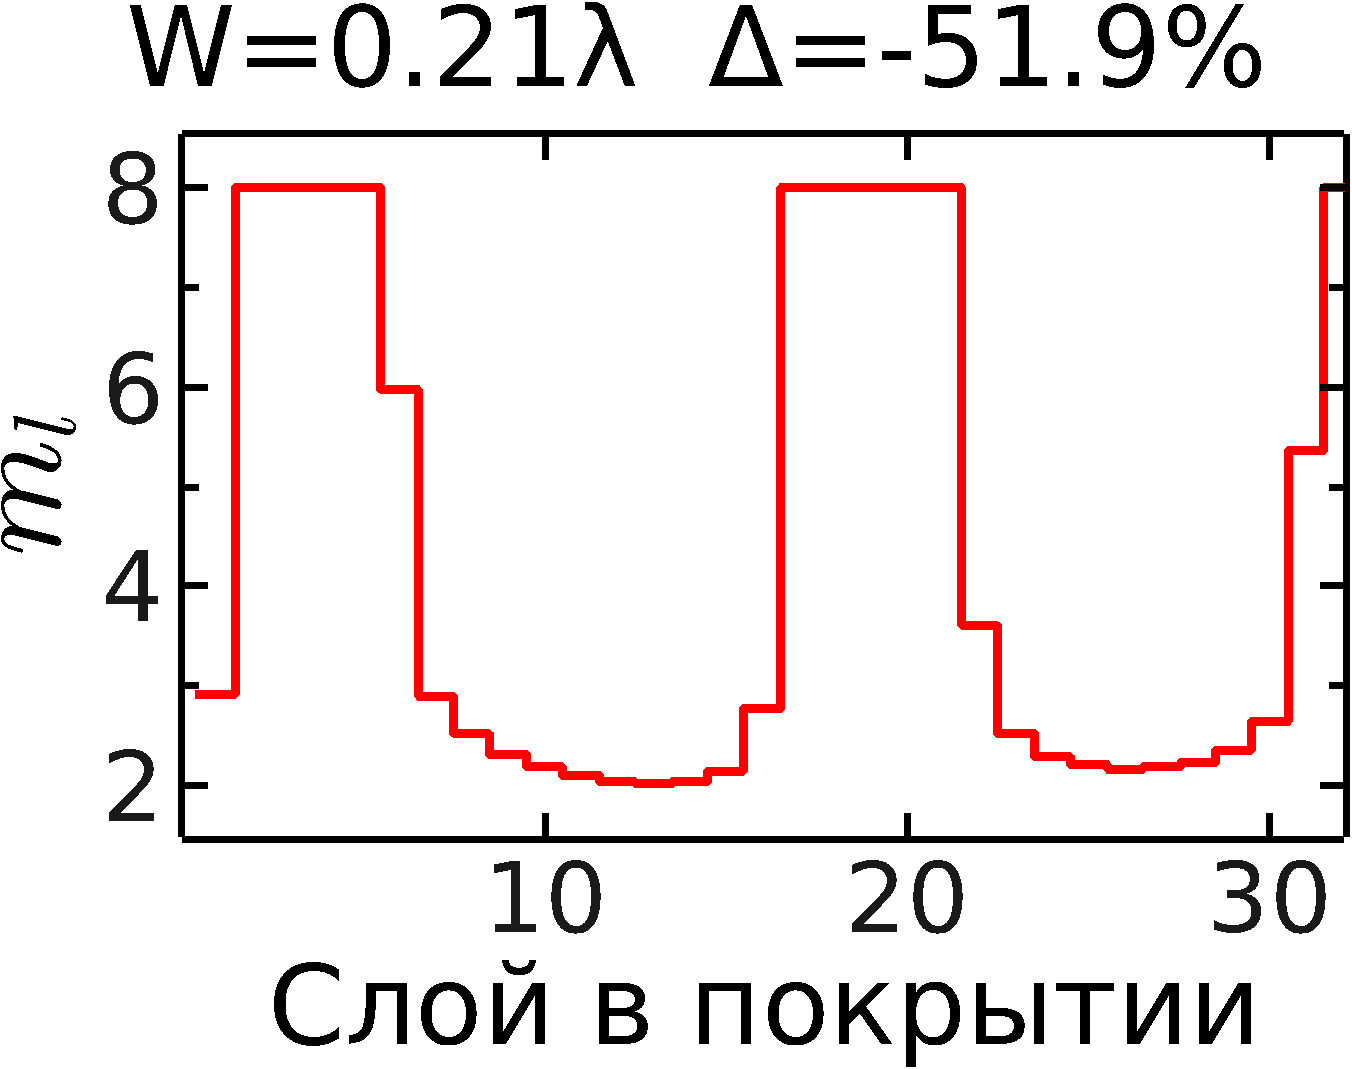
\includegraphics[width=0.95\linewidth]{w08-double-valley-index} \\ б)}
  \end{minipage}
  \hfill
  \begin{minipage}[ht]{0.32\linewidth}
    \center{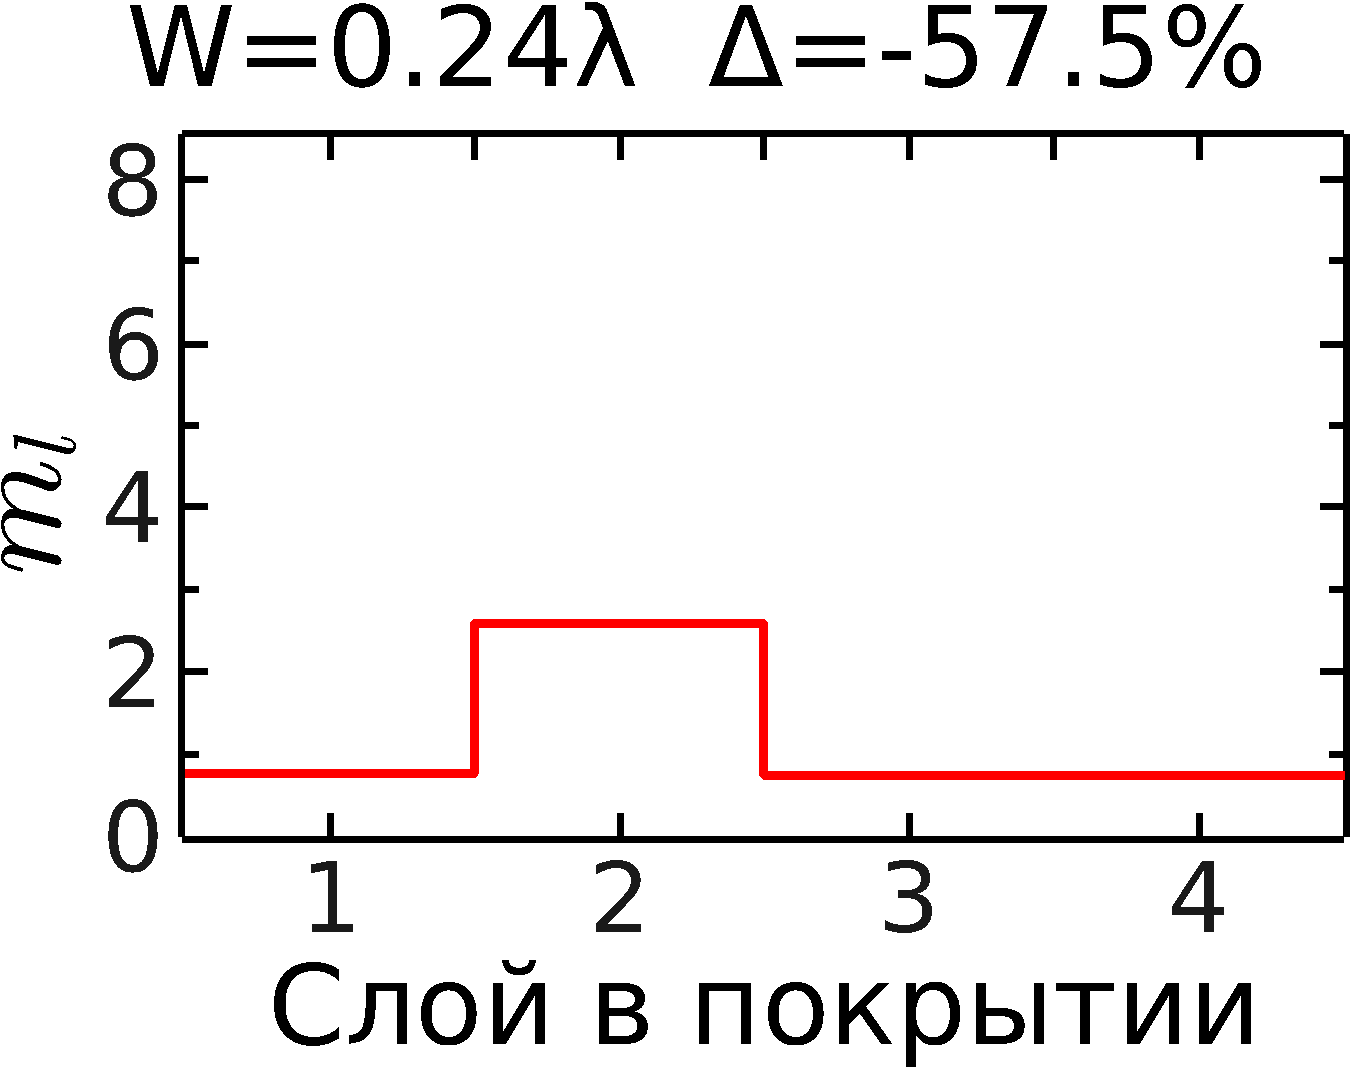
\includegraphics[width=0.95\linewidth]{index07-TO} \\ в)}
  \end{minipage}
  \caption{Типичные дизайны, обеспечивающие наилучшую маскировку при
    толщине покрытия, равной (a)~$0.11\lambda$, (б)~$0.21\lambda$ и
    (в)~$0.24\lambda$. Максимальное значение показателя преломления
    было ограничено $n_{\mathrm{max}}=8$, а минимальное значение
    было равно (а,б) $n_{\mathrm{min}}=1$ и (в) $n_{\mathrm{min}}=0.67$
  }
  \label{img:designs}  
\end{figure}
\begin{figure}[p]
  \begin{minipage}[ht]{0.495\linewidth}
    \center{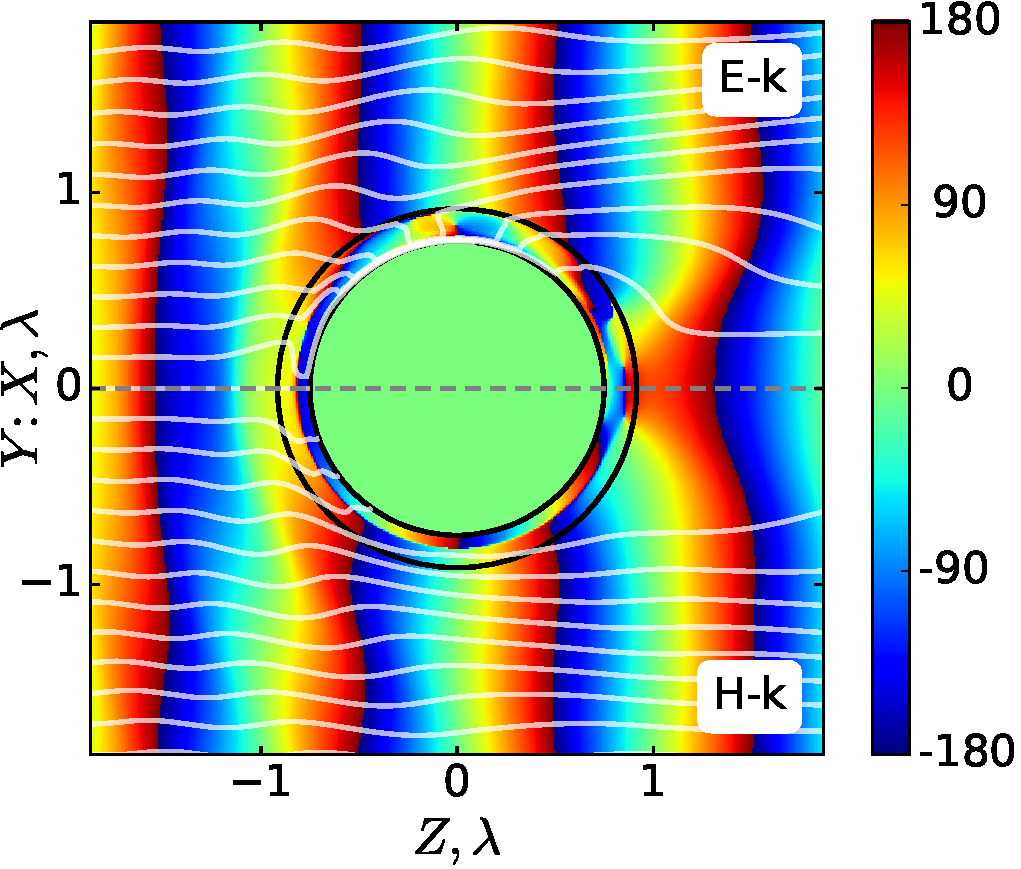
\includegraphics[width=0.98\linewidth]{PEC-index-sv-R3-XYZ-angleEx} \\ а)}
  \end{minipage}
  \hfill
  \begin{minipage}[ht]{0.495\linewidth}
    \center{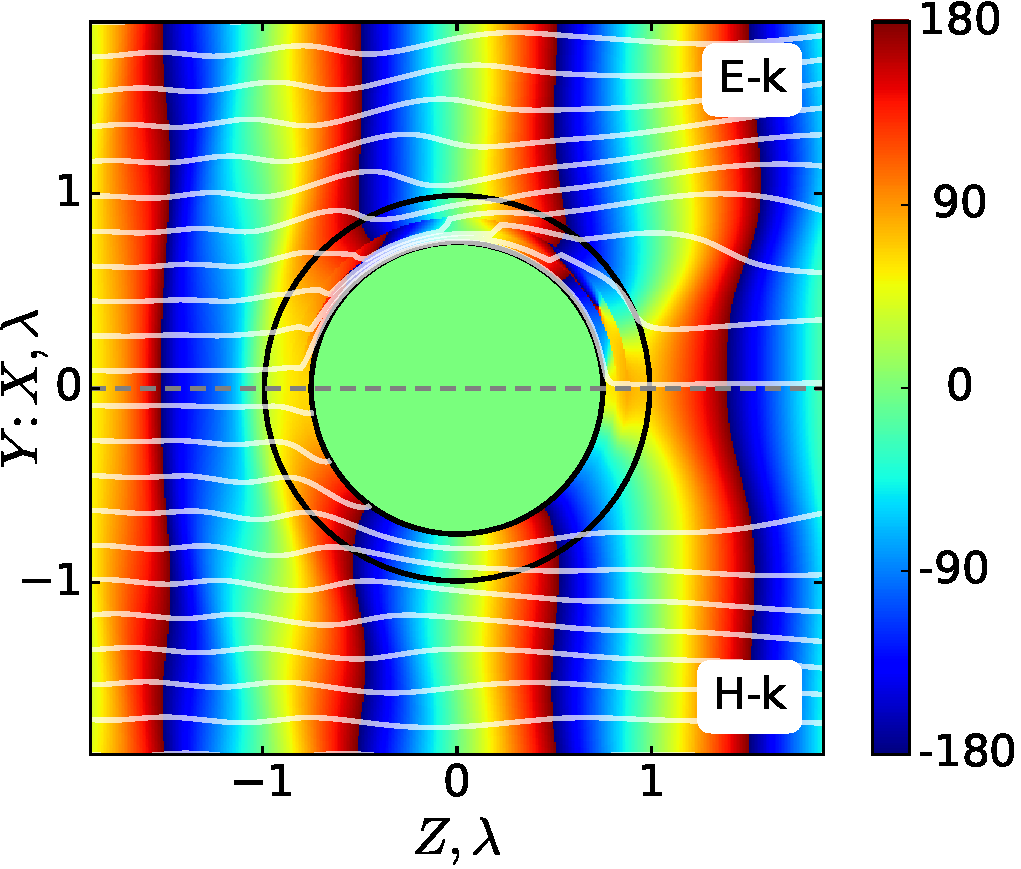
\includegraphics[width=0.98\linewidth]{PEC-index-in-glass-R1-XYZ-angleEx} \\ б)}
  \end{minipage}
  \caption{Изображение фазы электрического поля в случае маскировки
    объекта покрытием из изотропных (а) диэлектриков
    (см.~рисунок~\ref{img:designs}а) и (б) материалов с
    ${\varepsilon <1}$ (см.~рисунок~\ref{img:designs}в). Изображения
    построены в виде эпюра из плоскости поляризации падающей волны
    (верхняя половина) и перпендикулярной плоскости (нижняя
    половина). Чёрные окружности маркируют границы маскирующего
    покрытия. Белым обозначены линии потока энергии, волна
    распространяется в плоскости рисунка слева направо.}
  \label{img:field-phase}  
\end{figure}

Анализ этого и аналогичных графиков для других значений отношения
радиуса к длине волны позволил выявить ряд характерных
особенностей. Например, существует некое пороговое значение толщины,
после которого становится возможным стабильное получение дизайнов,
обеспечивающих заметное уменьшение сечения рассеяния. При этом
наилучшие показатели обеспечивают дизайны характерной структуры, где
несколько слоёв с высоким показателем преломления окружают группу
слоёв с низким показателем преломления. Увеличение общей толщины
покрытия приводит к переходу от дизайнов в одной такой группой
(рисунок~\ref{img:designs}а) к дизайнам с двумя группами
(рисунок~\ref{img:designs}б).

% ГОСТ Р 7.0.11—2011
% 5.3.9 На все иллюстрации должны быть приведены ссылки в тексте
% диссертации. При ссылке следует писать слово «Рисунок» с указанием
% его номера.

Сильной стороной теории Ми является возможность получать распределение
электрического и магнитного поля как внутри, так и вокруг изучаемой
наночастицы, вычислять значение фазы полей, а также строить линии
потока энергии.  Например, для структуры, изображённой на
рисунке~\ref{img:designs}а, было рассчитано распределение фазы
электрического поля в окружающем частицу пространстве и внутри
покрытия (рисунок~\ref{img:field-phase}а).  Из рисунка видно, что
волна, проходящая через маскирующее покрытие, испытывает задержку фазы,
приблизительно равную $2\pi$. Другими словами, такой дизайн приводит к
тому, что электромагнитная волна после распространения внутри покрытия
на выходе оказывается в фазе с волной, которая двигалась в окружающем
пространстве.  Это, в свою очередь, подавляет картину интерференции в
дальнем поле и, в конечном итоге, объясняет возникающий маскирующий
эффект.

Иначе выглядит распределение фазы электрического поля на
рисунке~\ref{img:field-phase}б, тут волна внутри покрытия на всей его
протяжённости движется в фазе с волной в окружающем пространстве. Это
стало возможным из-за использования в оптимизации материалов с
${\varepsilon<1}$, что соответствует маскировке объекта во вмещающей
среде, в которой скорость распространения света ниже, чем внутри
маскирующего покрытия.  Такие покрытия отличаются характерным дизайном
(рисунок~\ref{img:designs}в), в котором один слой с высоким
показателем преломления находится между слоями с ${\varepsilon<1}$.
\begin{figure}[t]
  \begin{minipage}[ht]{0.49\linewidth}
    \center{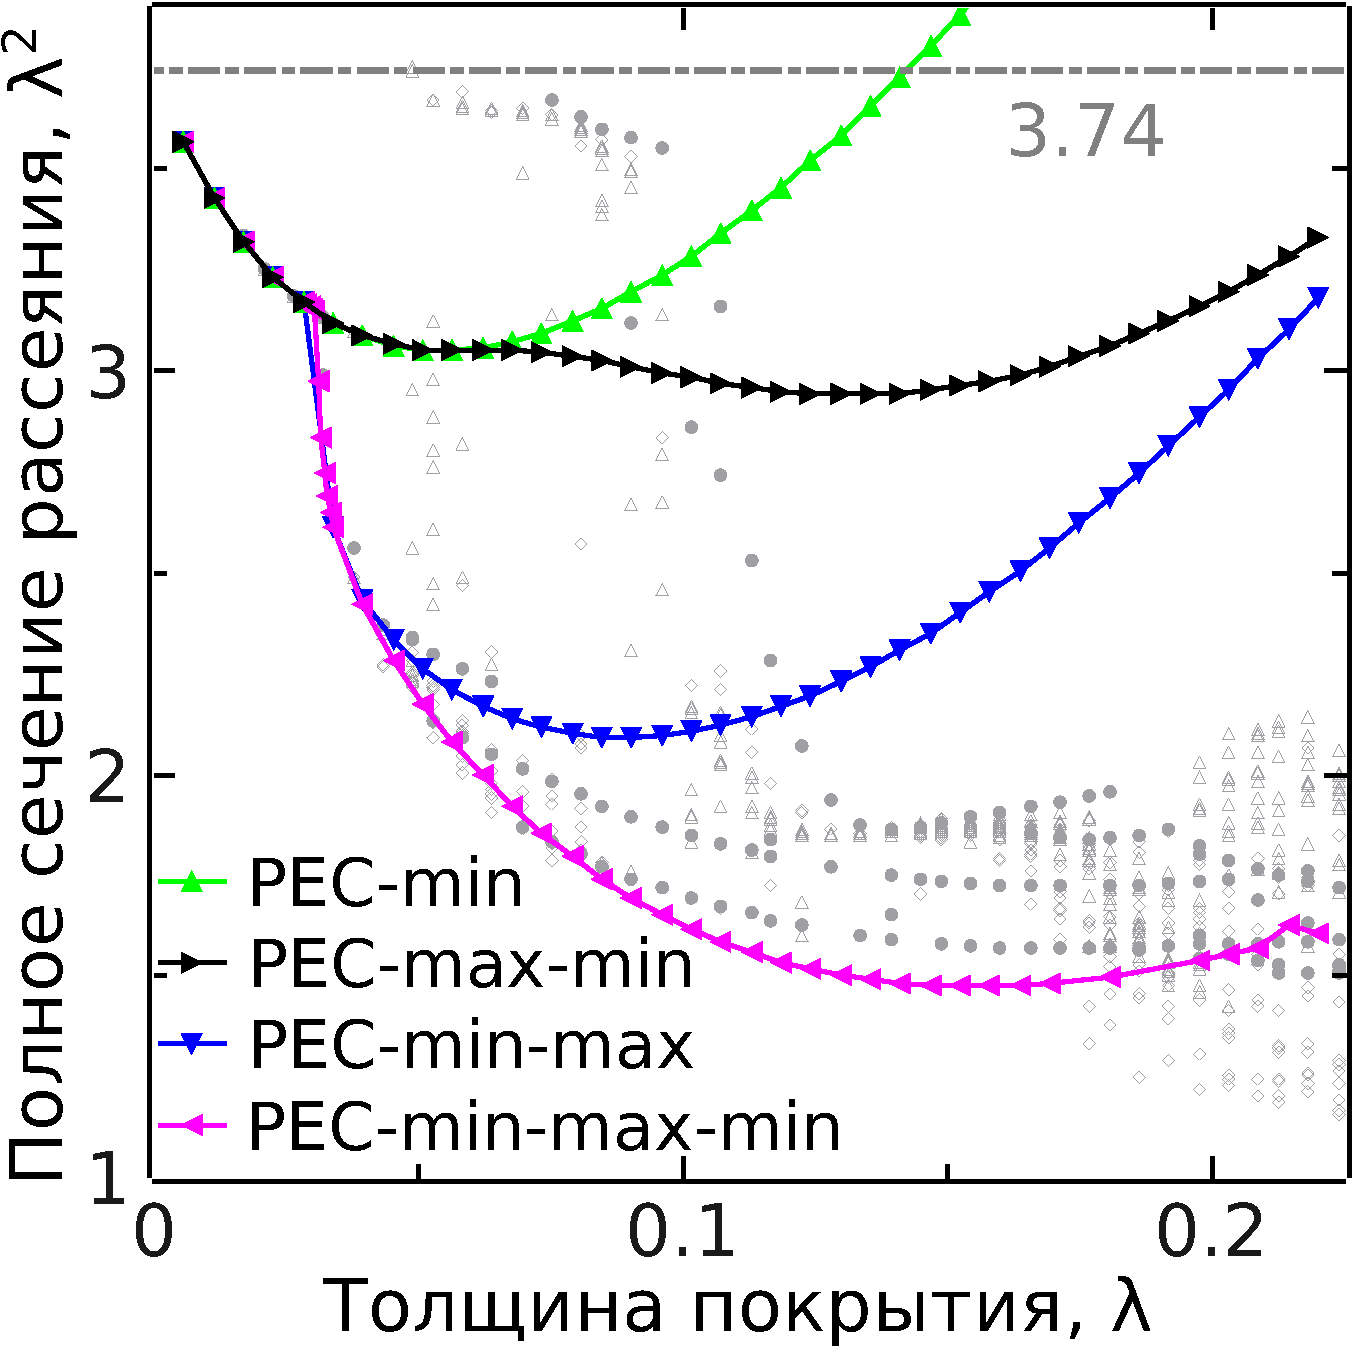
\includegraphics[width=0.95\linewidth]{rcs-overview-index07-DI} \\ а)}
  \end{minipage}
  \hfill
  \begin{minipage}[ht]{0.49\linewidth}
    \center{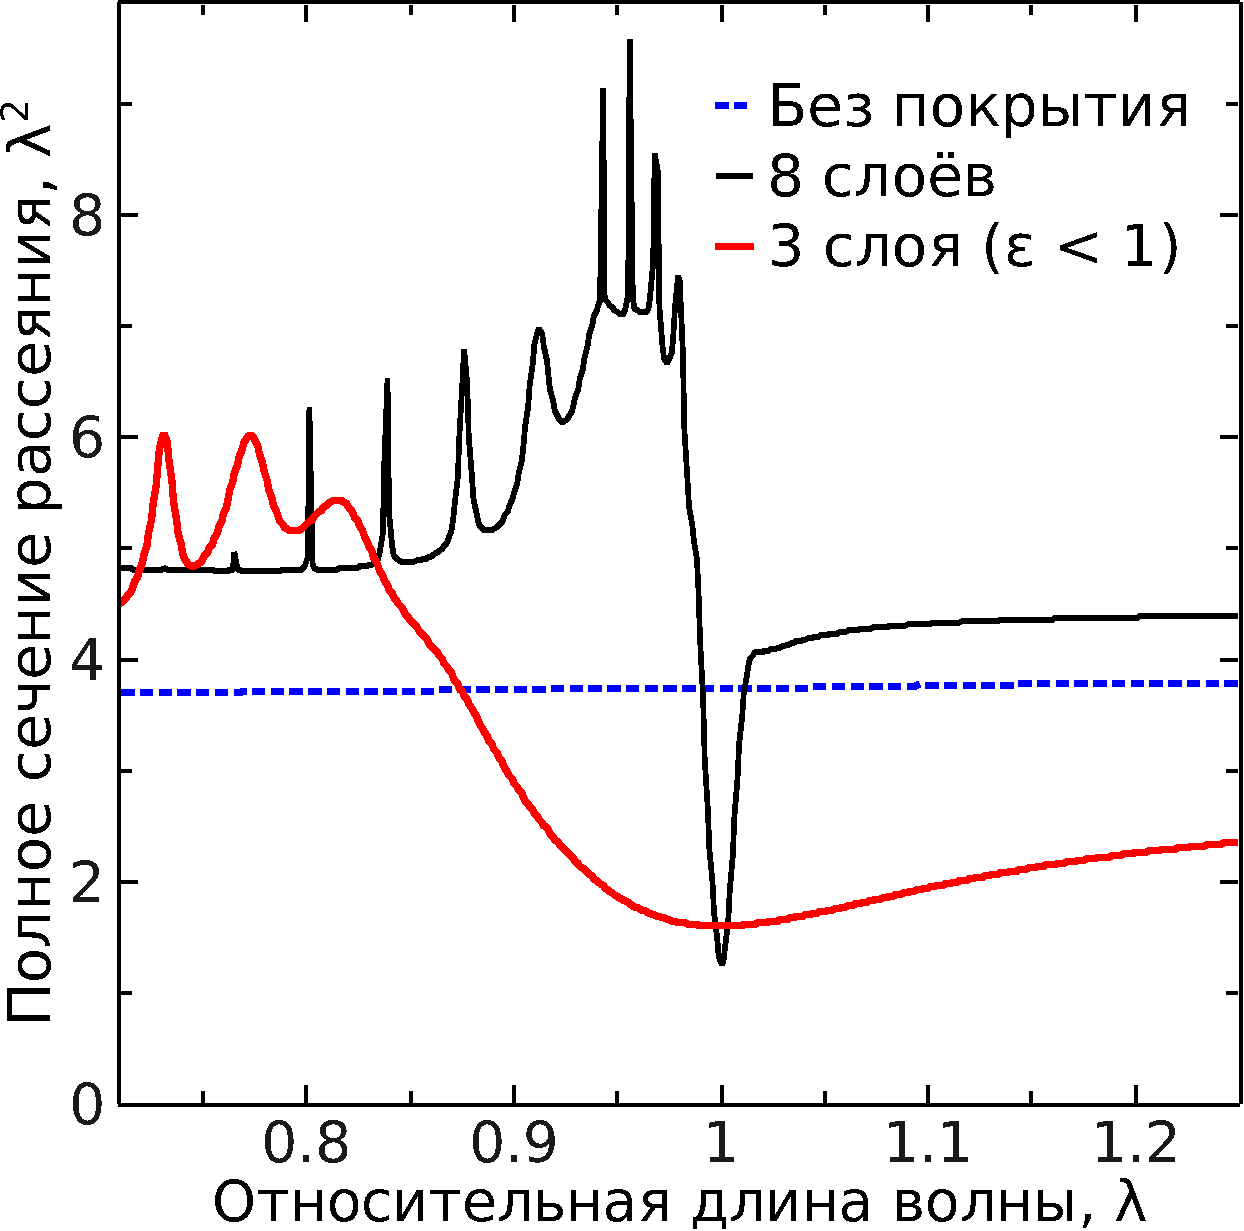
\includegraphics[width=0.95\linewidth]{index07-spectra} \\ б)}
  \end{minipage}
  \caption{а) Результат оптимизации покрытий с чередующимися слоями из
    большого $\varepsilon$ и ${\varepsilon<1}$. б) Спектры частицы
  без покрытия и с маскирующими покрытиями: из 8-ми слоёв диэлектрика и
  из 3-х слоёв с применением ${\varepsilon<1}$.}
  \label{img:min-max-min}  
\end{figure}

Обнаруженная закономерность позволила сформулировать гипотезу,
что для создания маскирующего покрытия достаточно использовать всего
два материала: с большим $\varepsilon$ и ${\varepsilon<1}$, а в
качестве параметров оптимизации можно использовать толщину каждого
слоя. Эта гипотеза была проверена численно, результаты оптимизации
отображены на рисунке~\ref{img:min-max-min}а. Оказалось, что для
большей части рассматриваемого диапазона общей толщины покрытия 
достаточно всего трёх слоёв, чтобы получить приблизительно то же
уменьшение полного сечения рассеяния, что и в случае применения 4, 8 и
16 слоёв равной толщины, когда при оптимизации
изменялись материальные параметры каждого слоя.

Особый интерес представляет различие в спектрах рассеяния для случаев
наличия и отсутствия материала с ${\varepsilon<1}$ в оптимизированном
покрытии.  При расчёте спектров для рисунка~\ref{img:min-max-min}б не
учитывалось наличие в материалах дисперсии и сопутствующих потерь,
поэтому их форма полностью определяется дизайном маскирующего
покрытия. Хорошо виден относительно узкий резонанс, который определяет
маскирующие свойства покрытия на основе диэлектриков. Использование
материала с ${\varepsilon<1}$ позволило в несколько раз расширить
диапазон длин волн, где наблюдается подавление рассеяния. 

\clearpage